\documentclass[a4paper, 12pt]{article}%тип документа

%отступы
\usepackage[left=2cm,right=2cm,top=2cm,bottom=3cm,bindingoffset=0cm]{geometry}

%Русский язык
\usepackage[T2A]{fontenc} %кодировка
\usepackage[utf8]{inputenc} %кодировка исходного кода
\usepackage[english,russian]{babel} %локализация и переносы

%Вставка картинок
\usepackage{wrapfig}
\usepackage{graphicx}
\graphicspath{{pictures/}}
\DeclareGraphicsExtensions{.pdf,.png,.jpg}

%оглавление
\usepackage{titlesec}
\titlespacing{\chapter}{0pt}{-30pt}{12pt}
\titlespacing{\section}{\parindent}{5mm}{5mm}
\titlespacing{\subsection}{\parindent}{5mm}{5mm}
\usepackage{setspace}

%Графики
\usepackage{multirow}
\usepackage{pgfplots}
\pgfplotsset{compat=1.9}

%Математика
\usepackage{amsmath, amsfonts, amssymb, amsthm, mathtools}

\begin{document}

\begin{titlepage}

\begin{center}
%\vspace*{1cm}
\large\textbf{Московский Физико-Технический Институт}\\
\large\textbf{(государственный университет)}
\vfill
\line(1,0){430}\\[1mm]
\huge\textbf{Работа 18}\\
\line(1,0){430}\\[1mm]
\vfill
\large Сибгатуллин Булат, ФРКТ\\
\end{center}

\end{titlepage}

\section*{ЗАДАНИЕ 1}

\begin{enumerate}

\item Соберем интегрирующую цепь и проведем измерения. Результаты запишем в таблицу:

\[C = 1 \quad \textit{мкФ}\]
\[R = 129 \quad (130) \quad \textit{Ом}\]
\[f_0 = 1000 \quad (1233) \quad \textit{Гц} \]

\begin{figure}[h!]
\centering
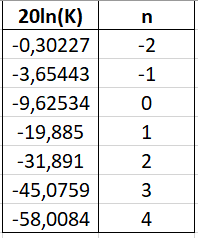
\includegraphics[scale=1]{table1.png}
\label{fig:Image1}
\end{figure}

Построим граф Боде для интегрирующий цепи по полученным данным:

\begin{figure}[h!]
\centering
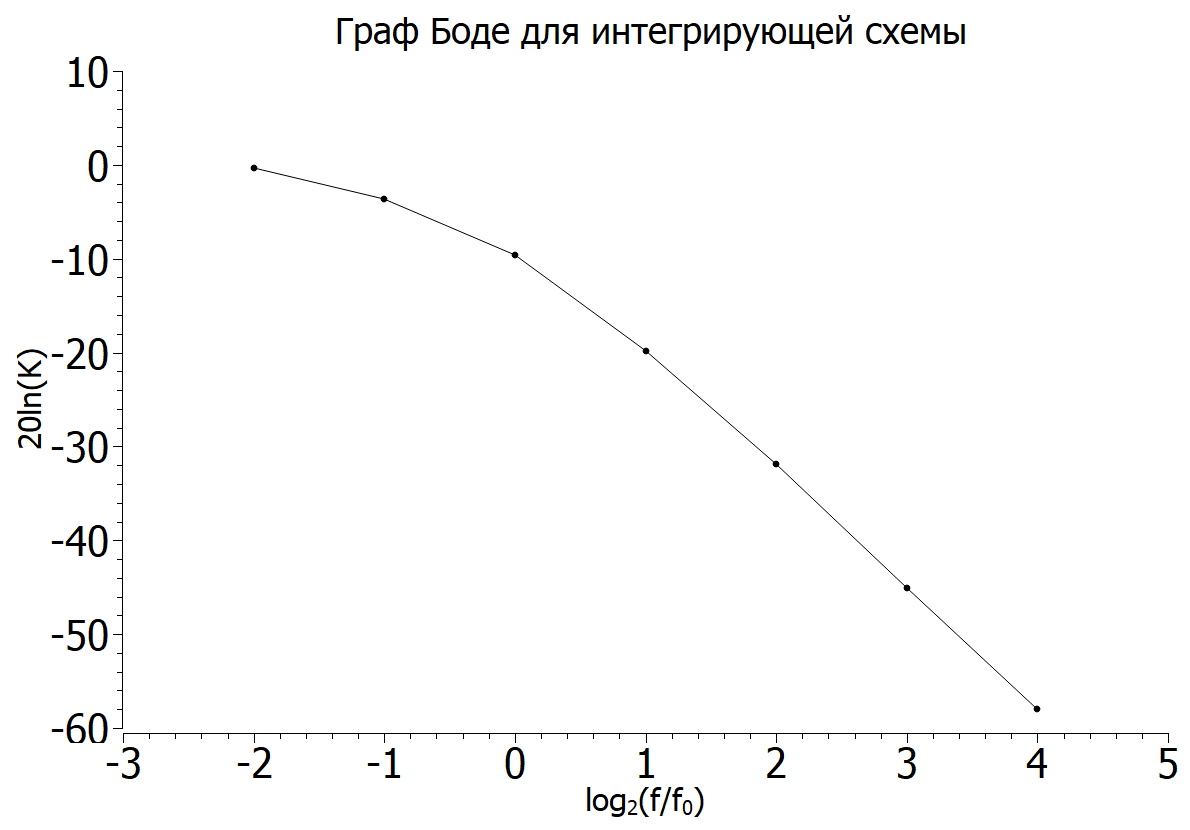
\includegraphics[scale=0.5]{graph1.png}
\label{fig:Image1}
\end{figure}

\item Подключим генератор прямоугольных сигналов. По осциллограме переходной характеристики оценим постоянную времени $\tau$:

\[\tau = 140 \quad \textit{мкс}\]

\[f_0 = \frac{1}{2\pi\tau} \approx 1 \quad \textit{кГц},\]

что совпадает со значеним для $f_0$ полученным в первом пункте.

\item Превратим интегрирующую цепь в дифференцирующую и проведем аналогичные измерения. Запишем результаты:

\[f_0 = 1 \quad \textit{кГц}\]

\begin{figure}[h!]
\centering
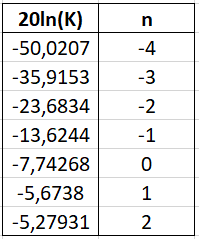
\includegraphics[scale=1]{table2.png}
\label{fig:Image1}
\end{figure}

Построим граф Боде для дифференцирующей цепи по полученным данным:

\begin{figure}[h!]
\centering
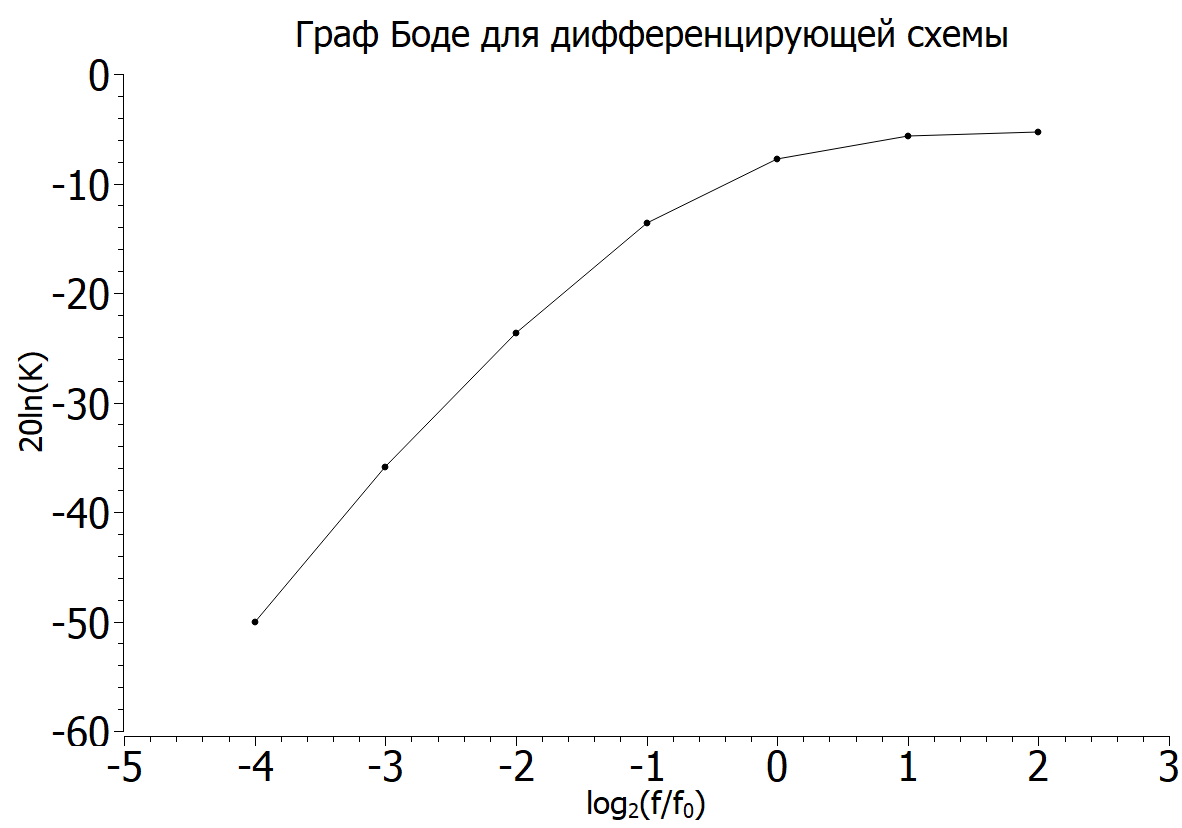
\includegraphics[scale=0.5]{graph2.png}
\label{fig:Image1}
\end{figure}

\item Подключим генератор прямоугольных сигналов. По осциллограме переходной характеристики оценим постоянную времени $\tau$:

\[\tau = 140 \quad \textit{мкс}\]

\[f_0 = \frac{1}{2\pi\tau} \simeq 1 \quad \textit{кГц},\]

что совпадает со значеним для $f_0$ полученным в первом пункте.

\item Откроем в MicroCap модель \textbf{rcint.cir}. Изучим графики частотной и фазовой характеристики.

\begin{figure}[h!]
\centering
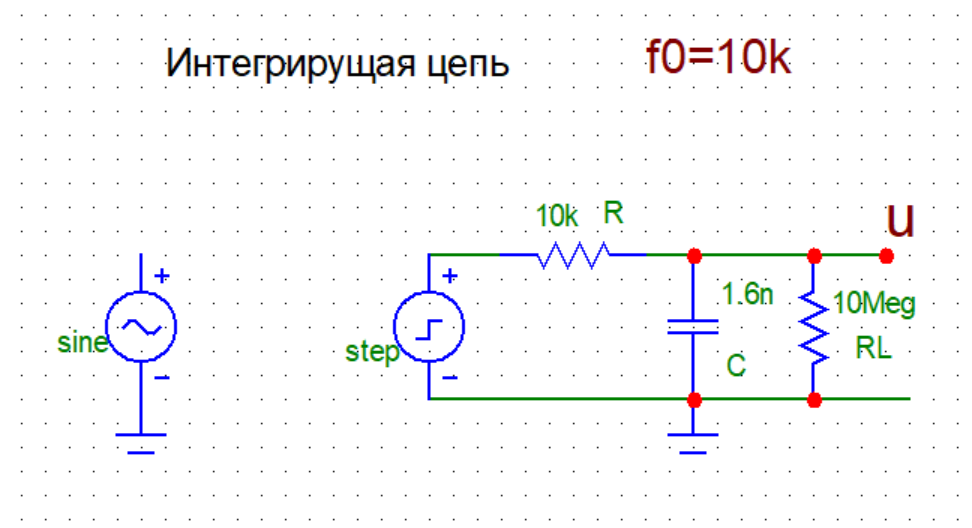
\includegraphics[scale=0.4]{rcint_img.png}
\label{fig:Image1}
\end{figure}

\begin{figure}[h!]
\centering
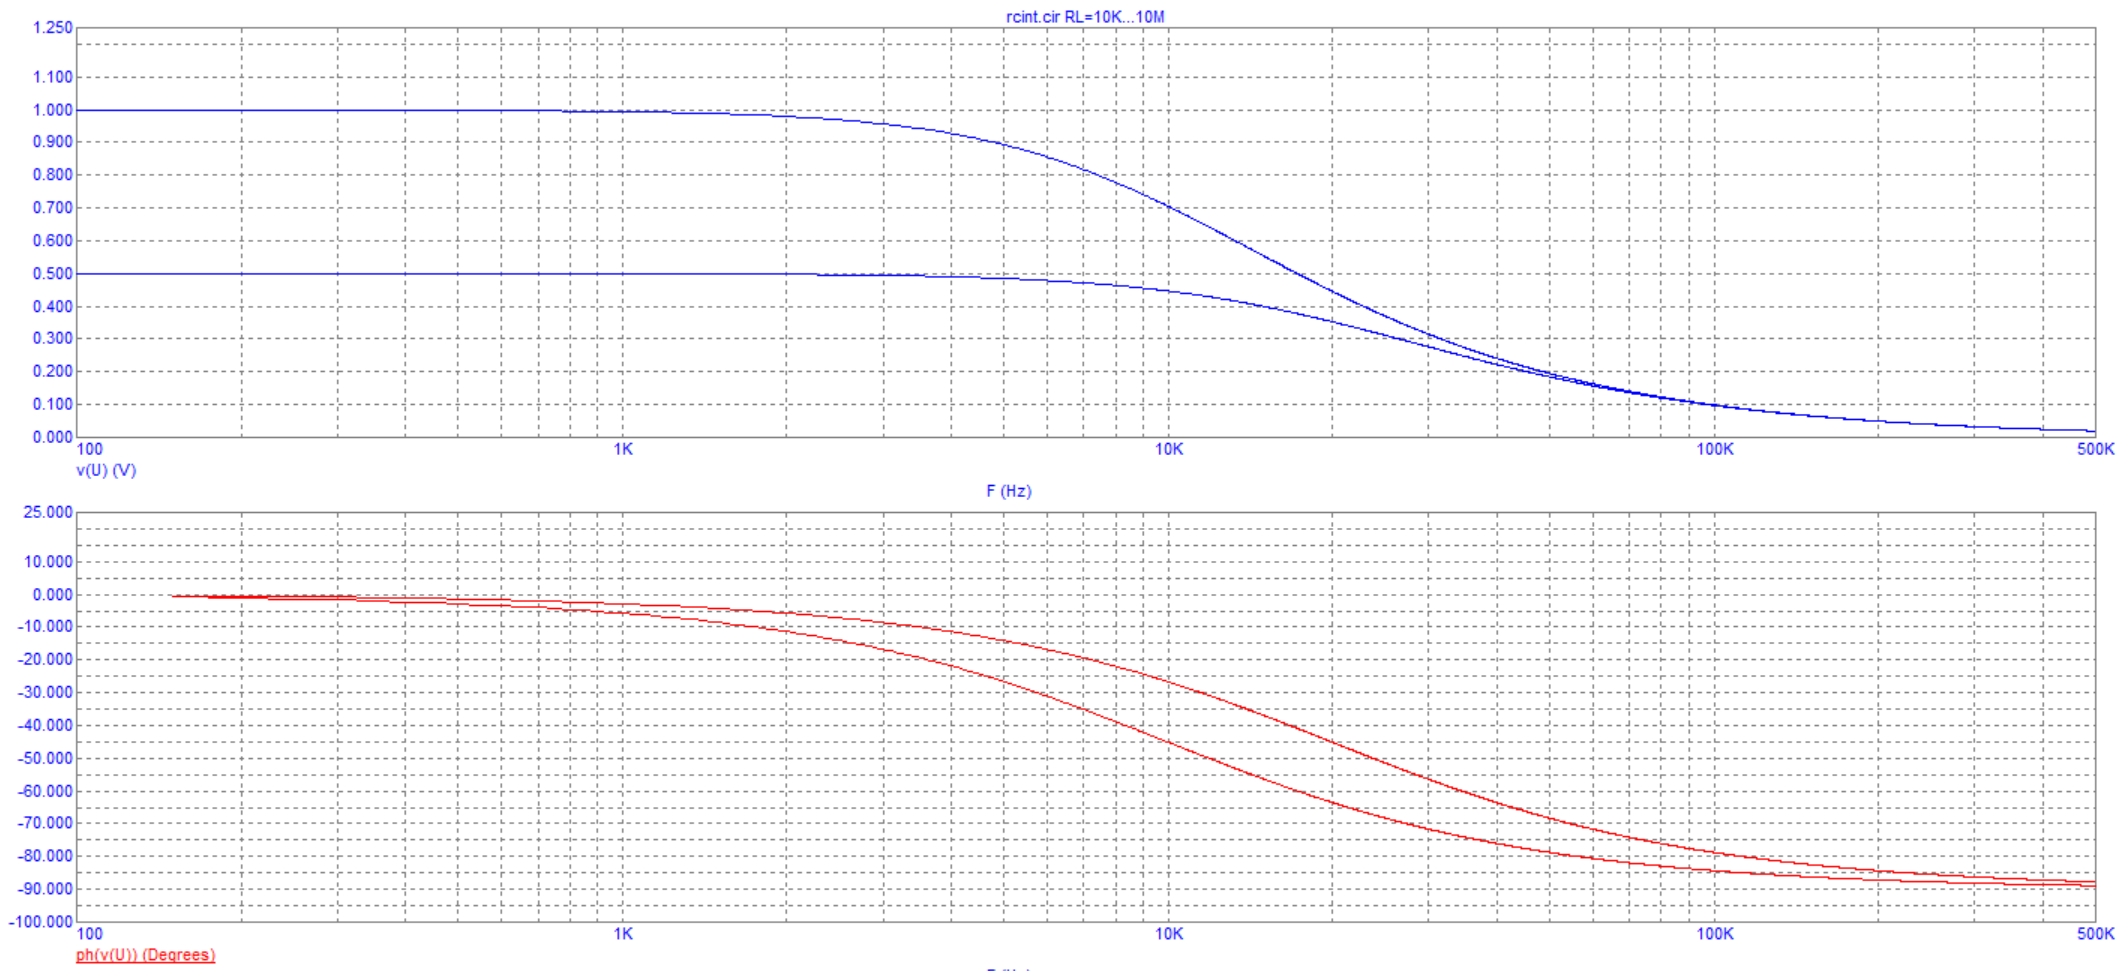
\includegraphics[scale=0.4]{rcint_AC.png}
\label{fig:Image1}
\end{figure}

По графику видно, что передаточная функция цепи принимает вид:

\[H(p) = \frac{K_0}{1 + p\tau}; \quad K_0 = \frac{R_L}{R + R_L},\tau = (R\Vert R_L) C.\]

По графику оценим верхнюю частоту:

\[R_L = 10 \: \textit{кОм}, \quad f_0 \simeq 10 \: \textit{кГц}\]
\[R_L = 10 \: \textit{МОм}, \quad f_0 \simeq 19,9 \: \textit{кГц}\]

Изучим переходную характеристику. По графику оценим постоянную времени:

\begin{figure}[h!]
\centering
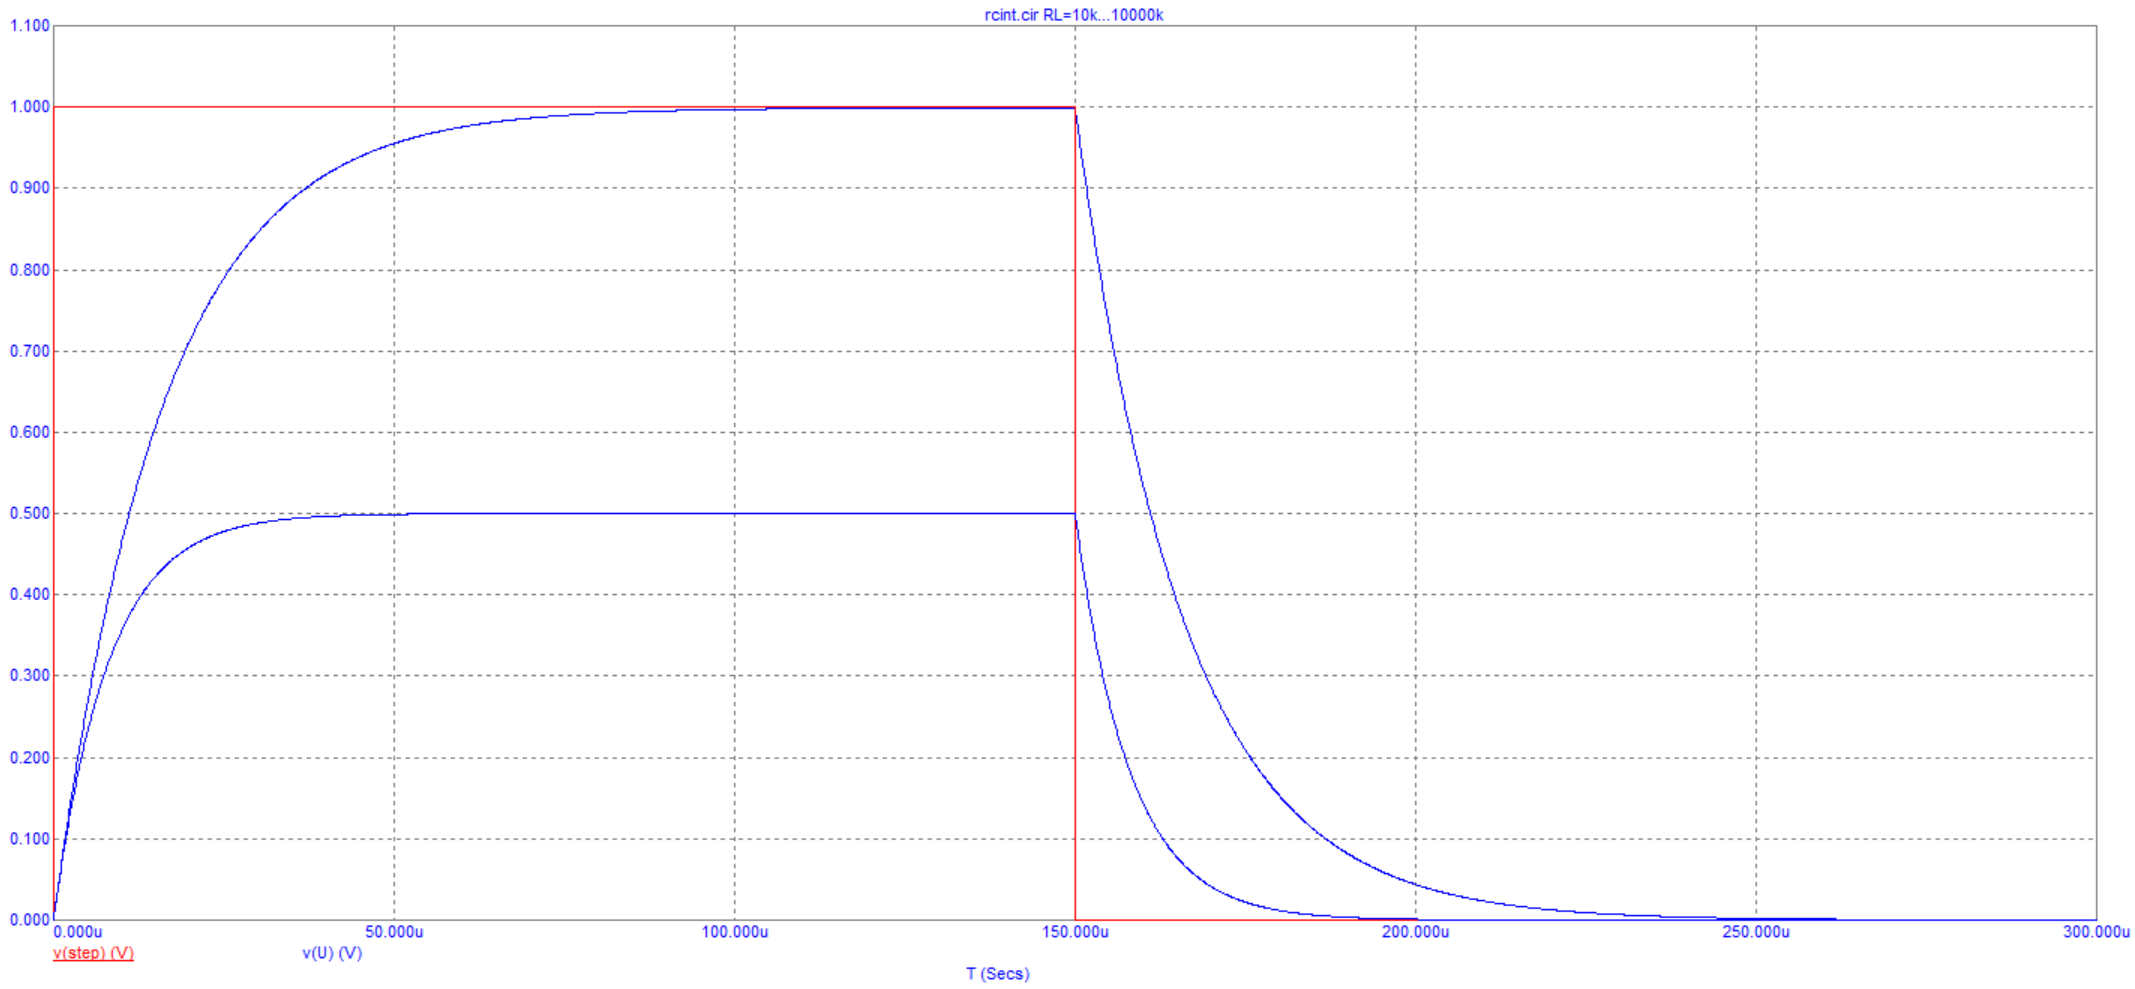
\includegraphics[scale=0.4]{rcint_Transient.png}
\label{fig:Image1}
\end{figure}

\[R_L = 10 \: \textit{кОм}, \quad \tau \simeq 9,7 \: \textit{мкс}\]
\[R_L = 10 \: \textit{МОм}, \quad \tau \simeq 19,6 \: \textit{мкс}\]

\item Откроем модель \textbf{rcdiff.cir}. Изучим ее частотную и фазовую характеристики.

\begin{figure}[h!]
\centering
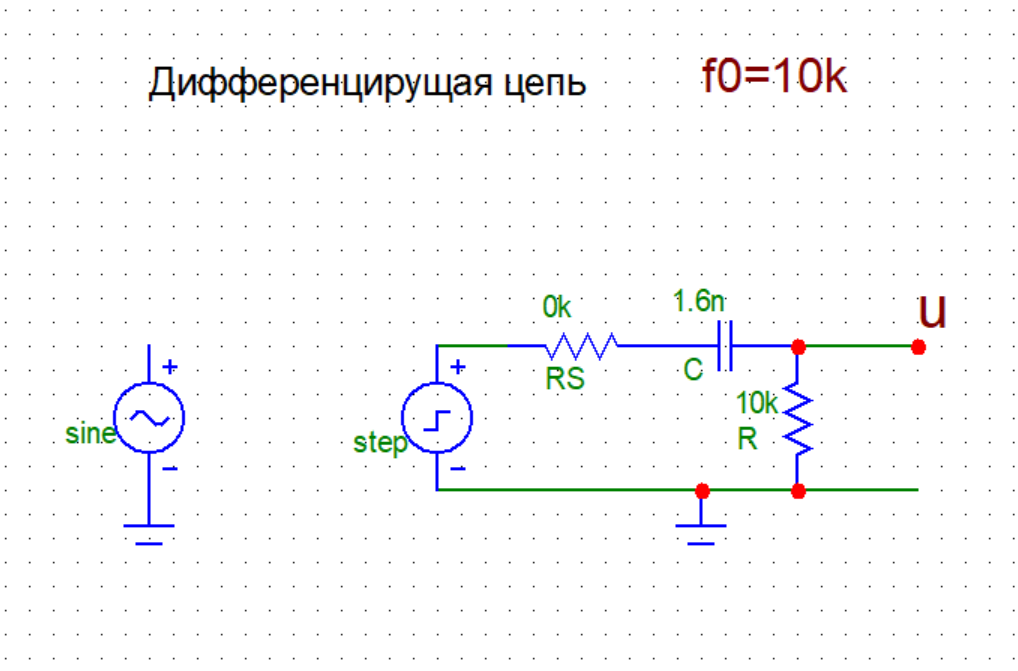
\includegraphics[scale=0.4]{rcdiff_img.png}
\label{fig:Image1}
\end{figure}

\begin{figure}[h!]
\centering
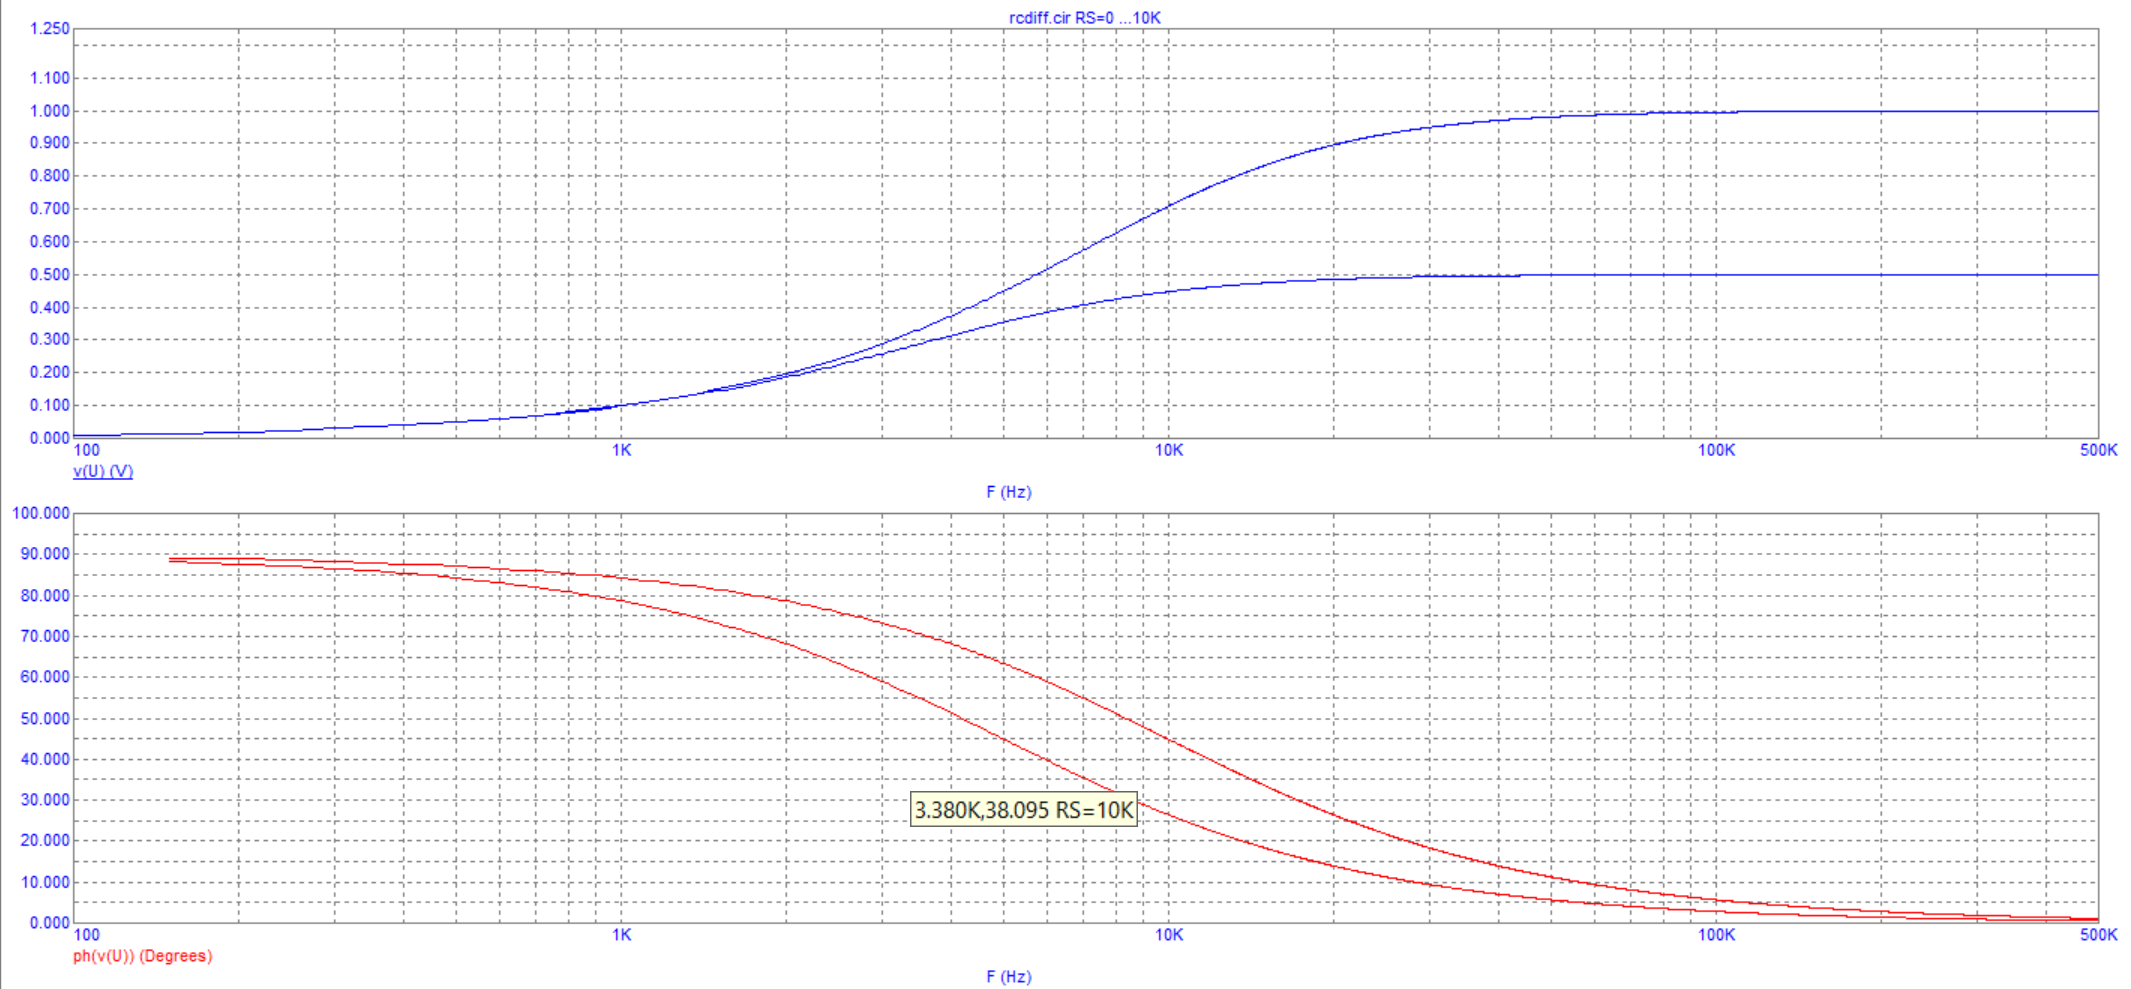
\includegraphics[scale=0.4]{rcdiff_AC.png}
\label{fig:Image1}
\end{figure}

По графику видно, что передаточная функция цепи при $R_S \neq 0$ принимает вид:

\[H(p) = \frac{K_0p\tau}{1 + p\tau}; \quad K_0 = \frac{R}{R + R_S},\tau = (R + R_S) C.\]

По графику оценим верхнюю частоту:

\[R_S = 0 \quad f_0 \simeq 9,75 \: \textit{кГц}\]
\[R_S = 10 \: \textit{кОм}, \quad f_0 \simeq 4,88 \: \textit{кГц}\]

Изучим переходную характеристику. По графику оценим постоянную времени:

\begin{figure}[h!]
\centering
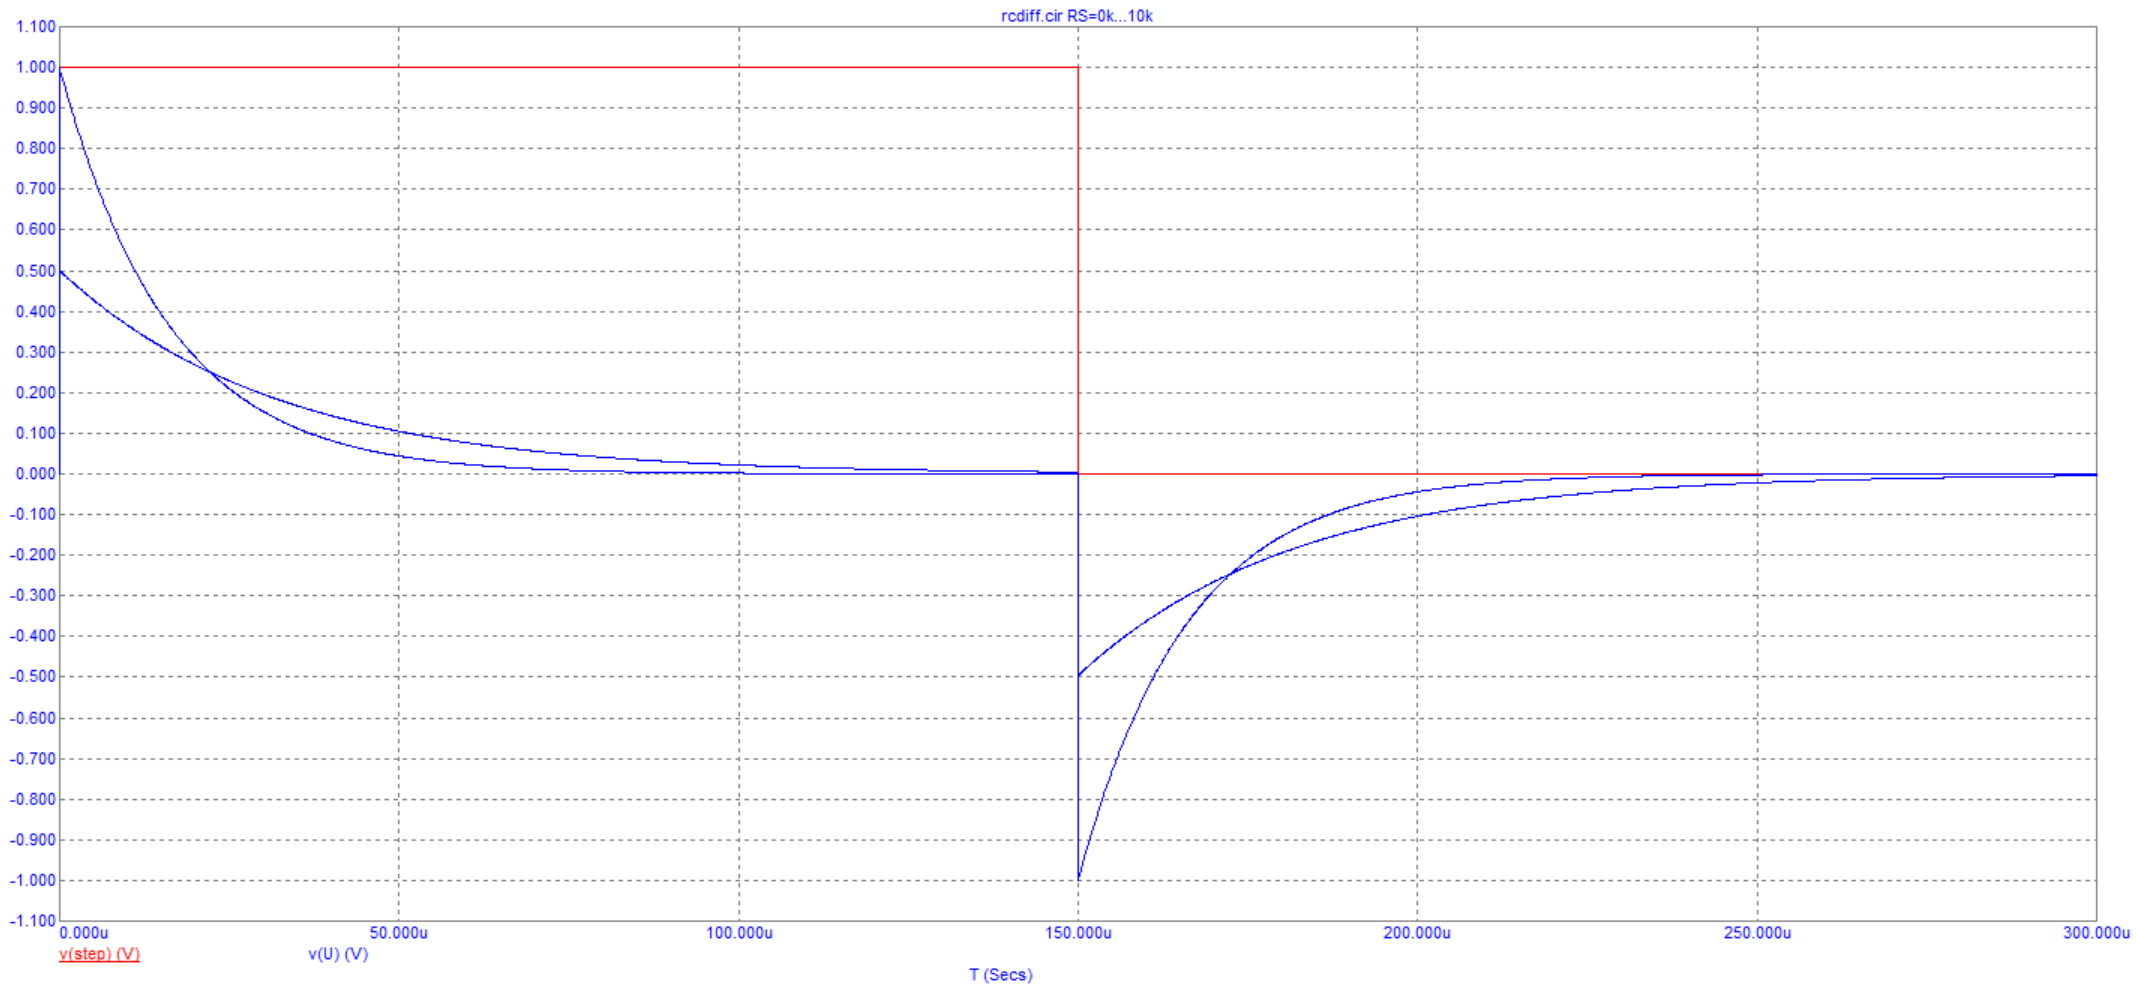
\includegraphics[scale=0.4]{rcdiff_Transient.png}
\label{fig:Image1}
\end{figure}

\[R_S = 0, \quad \tau \simeq 16,7 \: \textit{мкс}\]
\[R_S = 10 \: \textit{кОм}, \quad \tau \simeq 31,8 \: \textit{мкс}\]

\item Откроем модель \textbf{rcpower.cir}. Изучим графики частотной зависимости потребляемых интегрирующей цепью активных и реактивных мощностей и графики мощностей на её комопонентах.

\begin{figure}[h!]
\centering
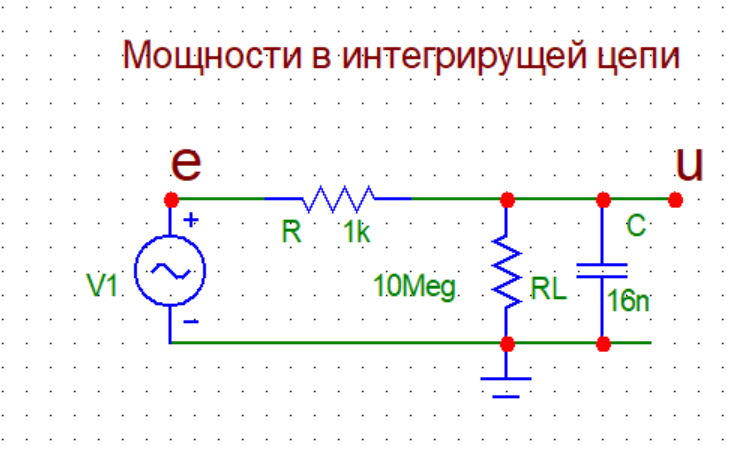
\includegraphics[scale=0.4]{rcpower_img.png}
\label{fig:Image1}
\end{figure}

\begin{figure}[h!]
\centering
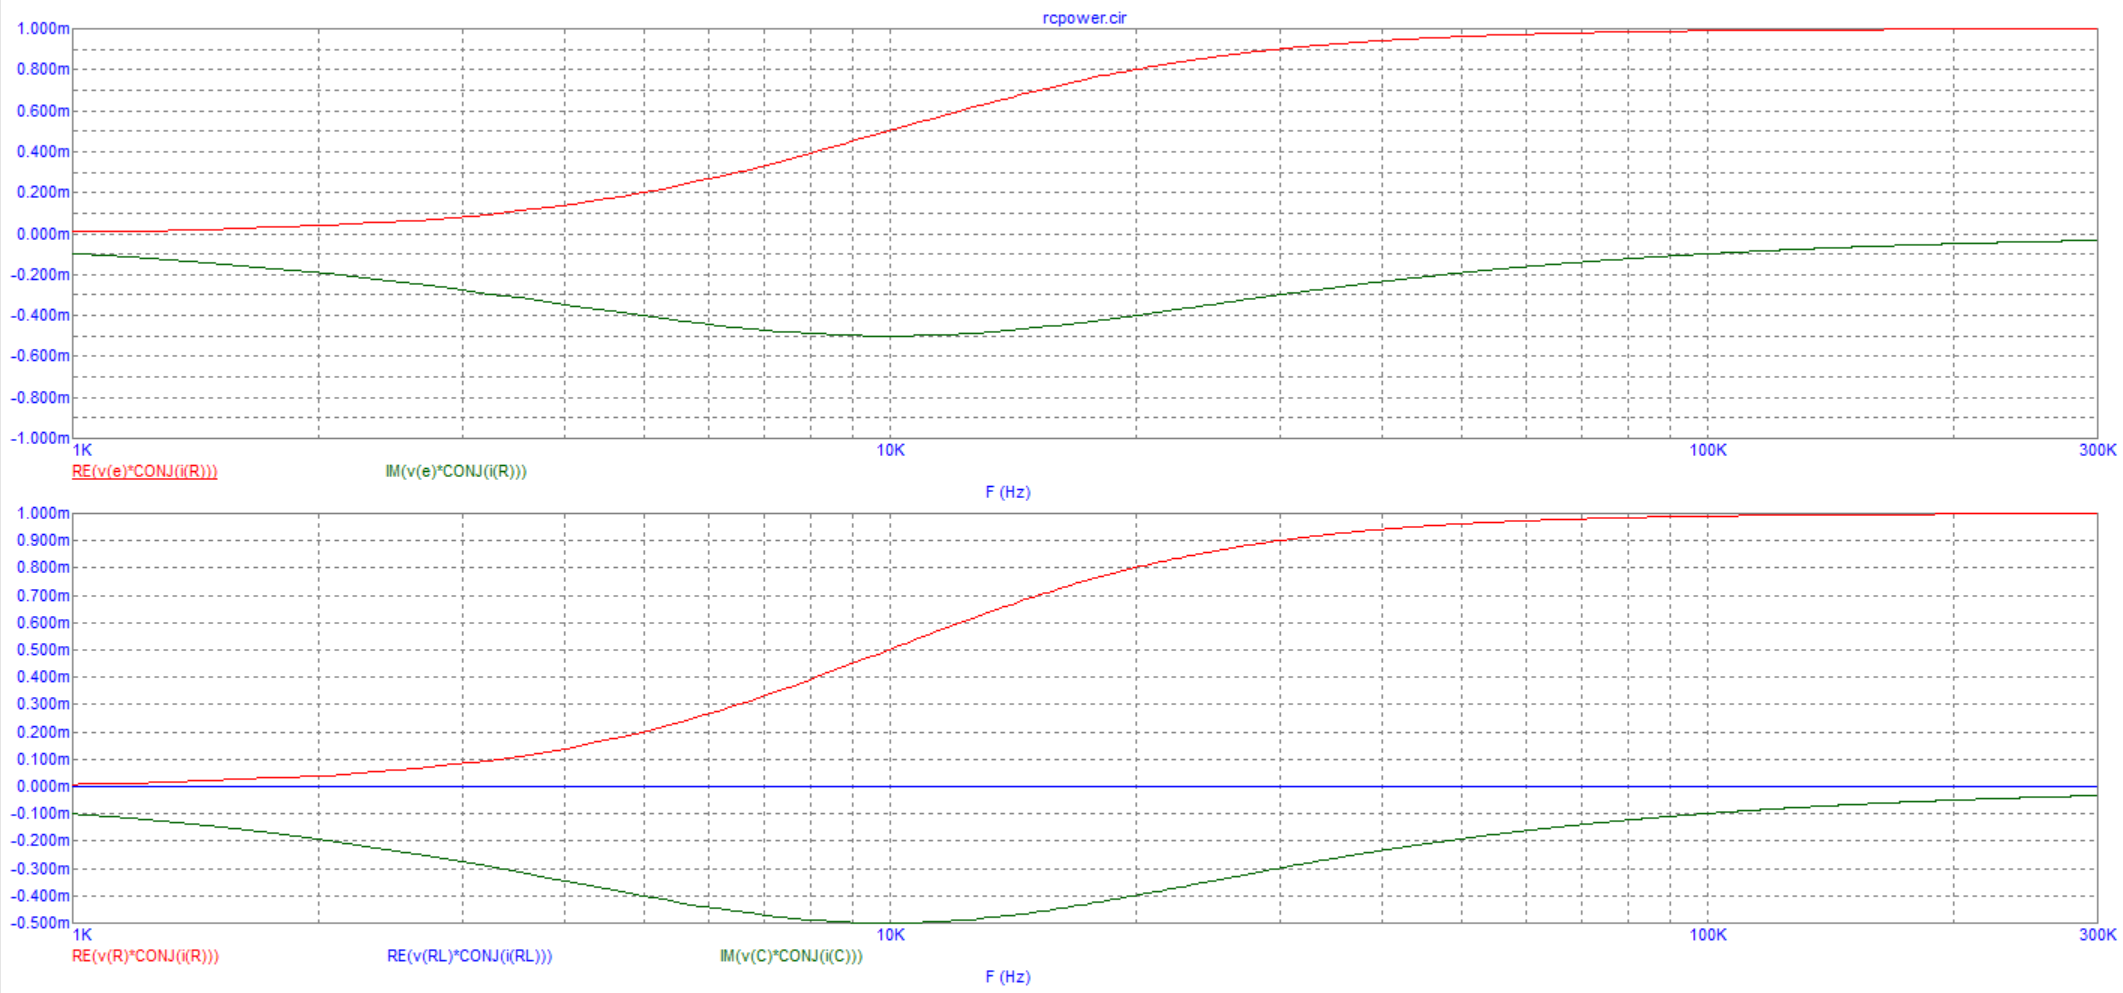
\includegraphics[scale=0.4]{rcpower_AC1.png}
\label{fig:Image1}
\end{figure}

Видно, что у реактивной компоненты потребление становится максимальным при частоте $f_0 = 10 \: \textit{кГц}$, и стремится к нулю при частоте $f = 0$ и $f = \infty$. При $f = f_0$ выполняется закон сложения мощностей.

Подключая и отключая резитор $R_L$ варьированием $[1k, 1Meg \vert 1Meg] (1Meg = \infty)$, изучим его влияние на распределение мощностей в схеме при $f = f_0$.

\begin{figure}[h!]
\centering
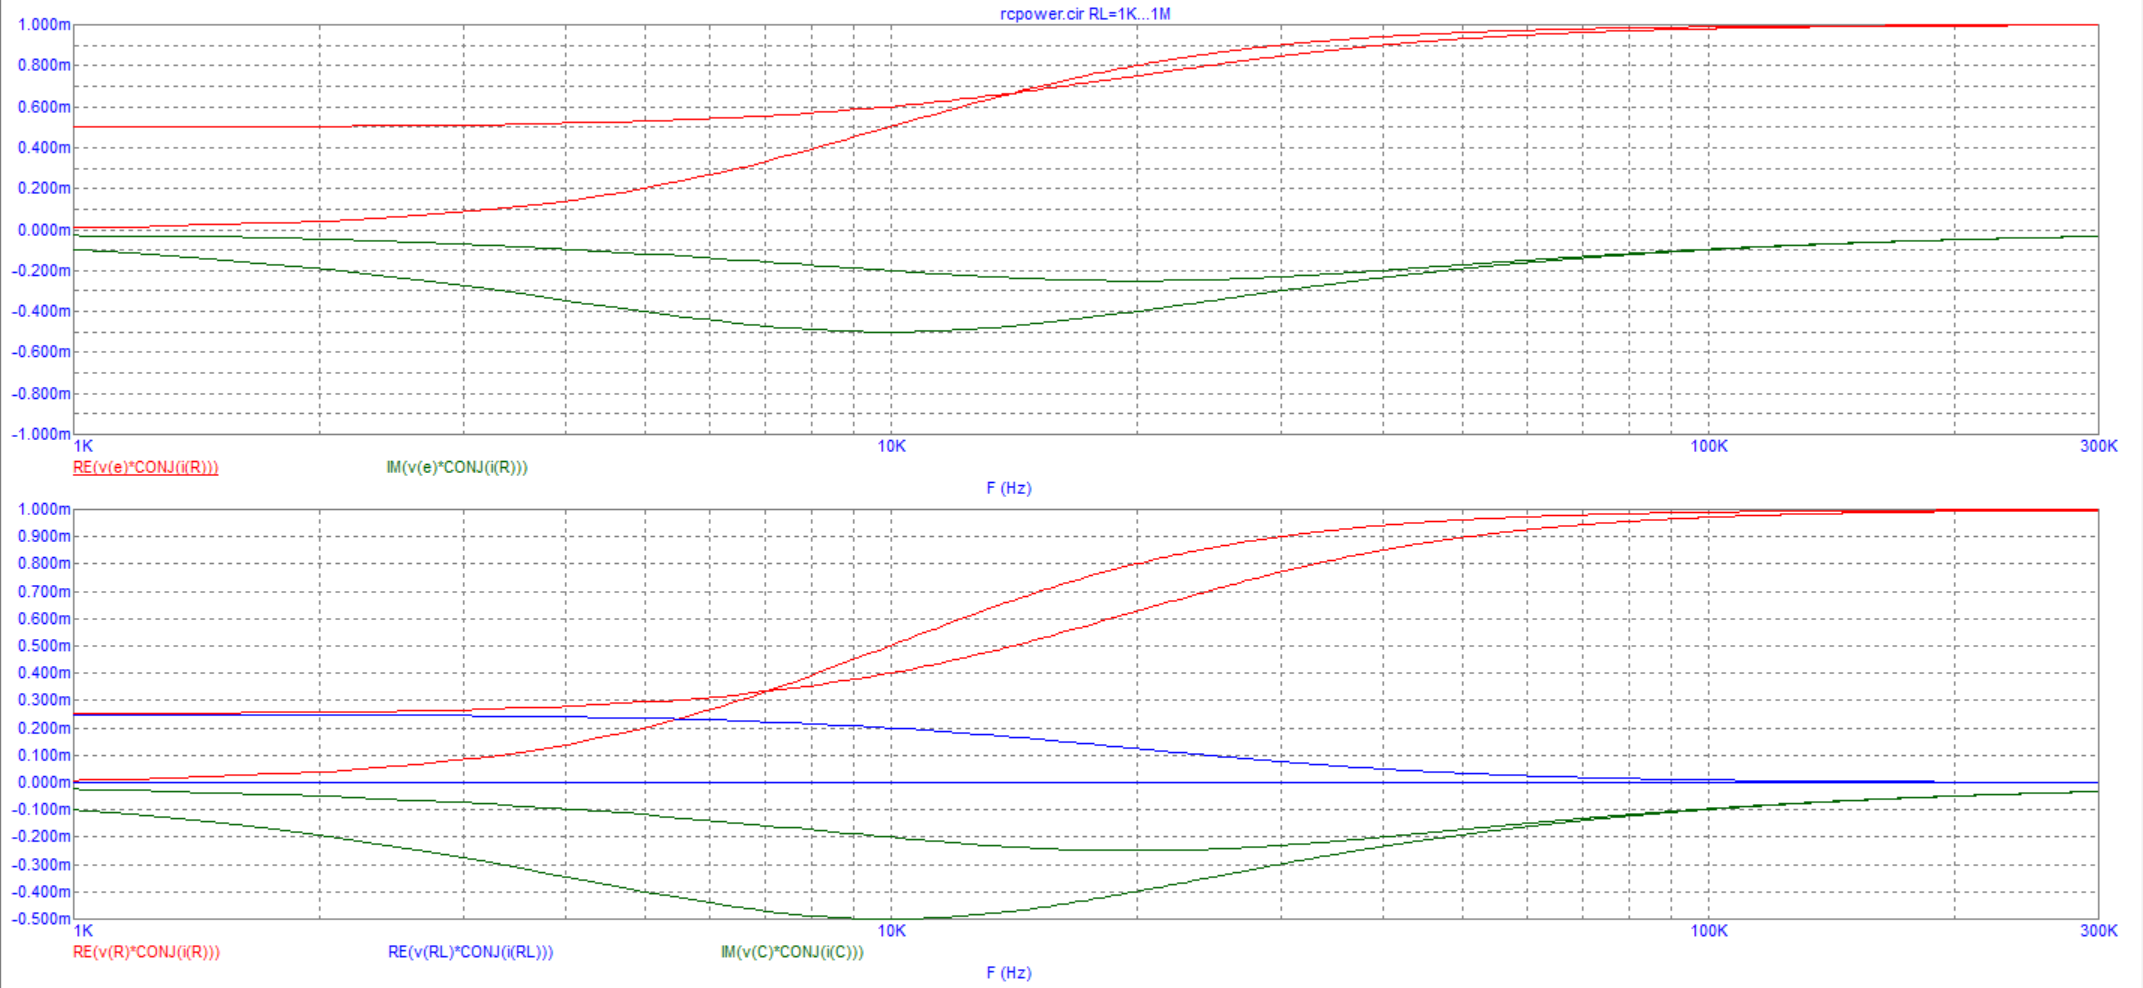
\includegraphics[scale=0.4]{rcpower_AC2.png}
\label{fig:Image1}
\end{figure}

При уменьшении значения сопротивления резистора $R_L$, его мощность возрастает до 0,2 \textit{мВт}, мощность на резисторе $R$ падает до 0,4 \textit{мВт}, а реактивная мощность конденсатора . Скорость увеличения мощности на резисторе $R_L$ становится равной -0,2 \textit{мВт}.

\end{enumerate}

\section*{ЗАДАНИЕ 2}

\begin{enumerate}

\item Откроем модель \textbf{rc2pole.cir}. 

\begin{figure}[h!]
\centering
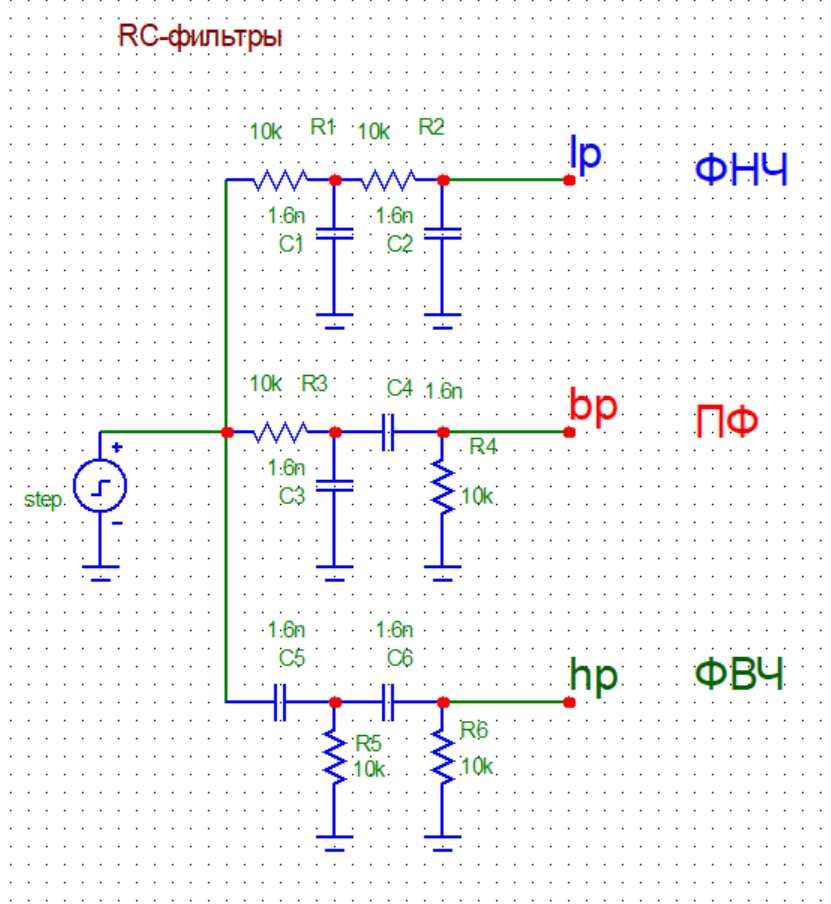
\includegraphics[scale=0.4]{rc2pole_img.png}
\label{fig:Image1}
\end{figure}

\begin{figure}[h!]
\centering
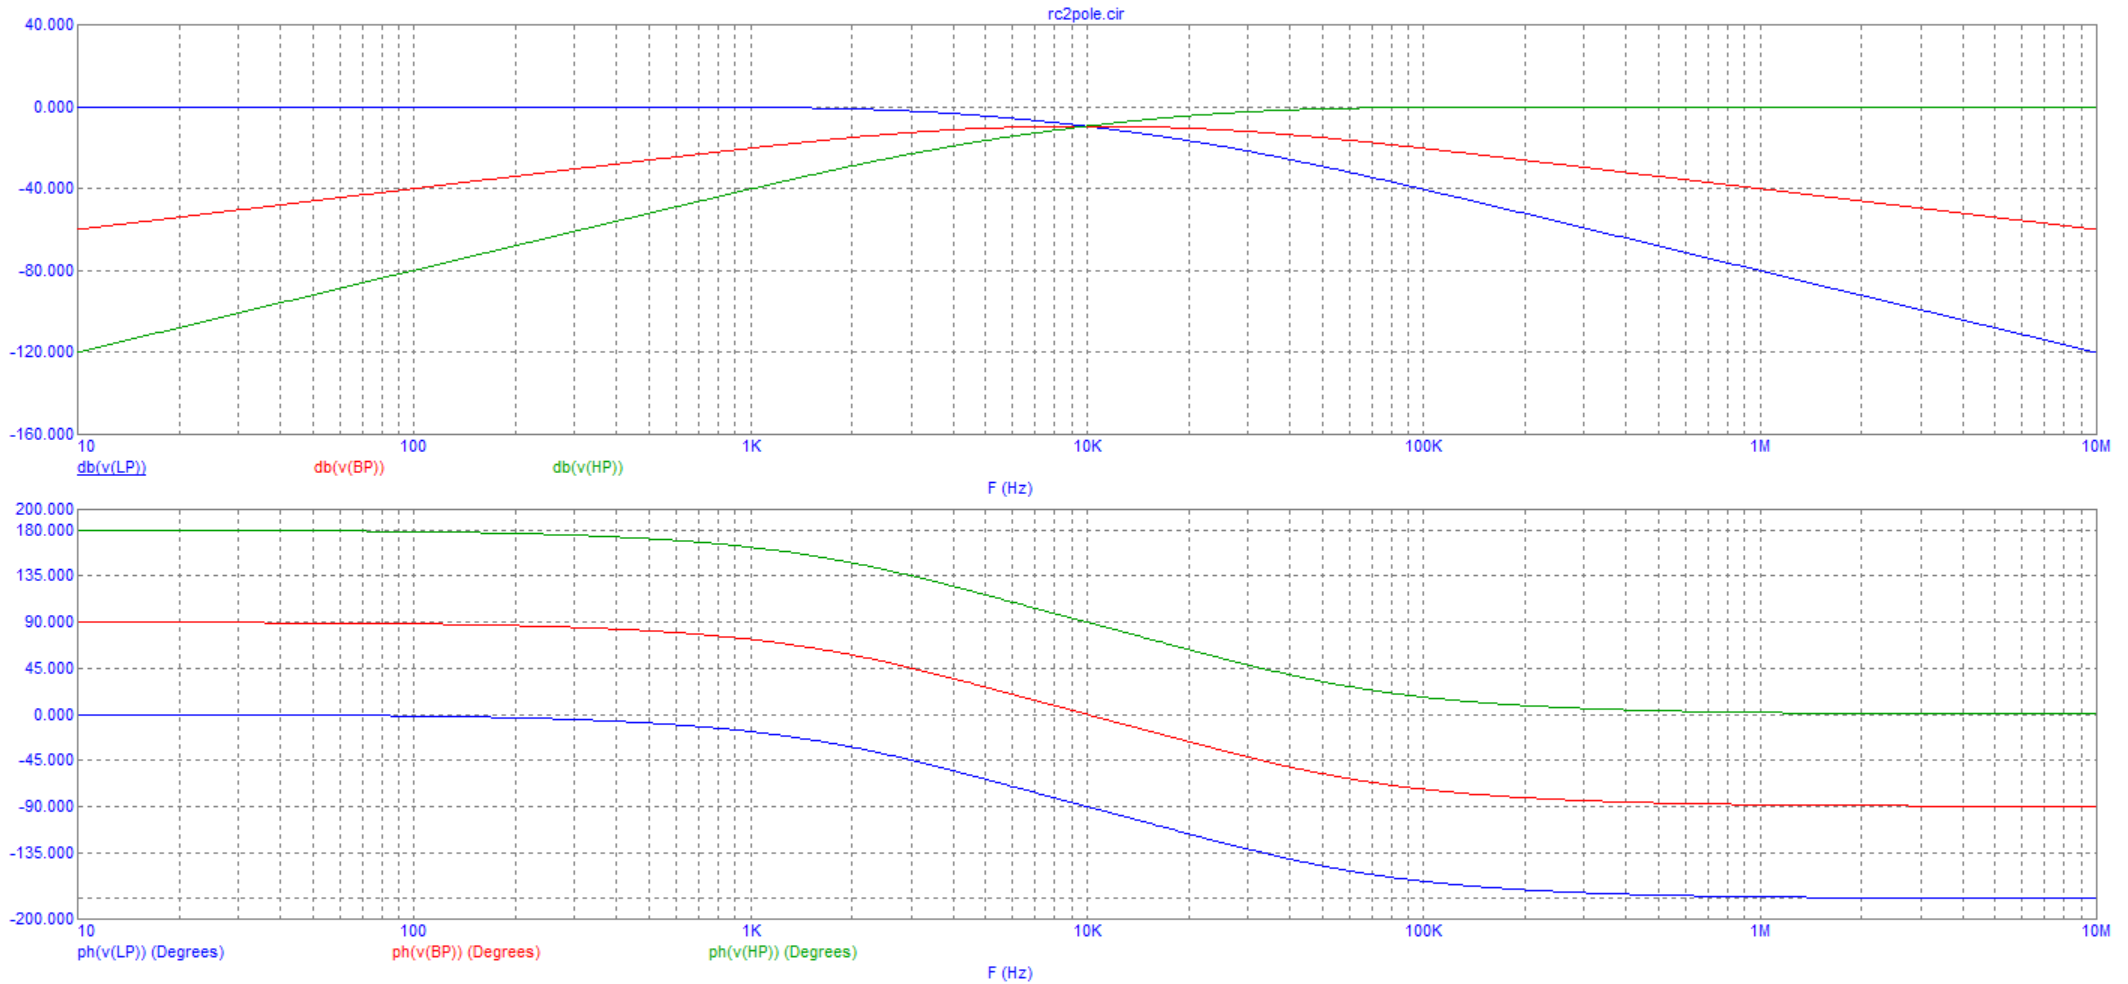
\includegraphics[scale=0.4]{rc2pole_AC.png}
\label{fig:Image1}
\end{figure}

По графикам определим затухание на частоте $f_0 \simeq 10 \: \textit{кГц}$, оно равно -9,6 \textit{dB} и скорость его нарастания в полосах задержания -40,4 + 9,6 = -30,8 \textit{dB}/\textit{декаду}. По графикам  ФЧХ измерим значения фазовых сдвигов  ФВЧ, ПФ и ФНЧ на частотах 0, $f_0$, $\infty$.

\begin{center}
\begin{tabular}{|c|c|c|c|}
\hline 
 & ФВЧ & ПФ & ФНЧ \\ 
\hline 
0 & 180 & 90 & 0 \\ 
\hline 
$f_0$ & 90 & 0 & -90 \\ 
\hline 
$\infty$ & 0 & -90 & -180 \\ 
\hline 
\end{tabular} 
\end{center}

Двухсторонняя полоса $\triangle f$ пропускания ПФ $\approx$ 30 \textit{кГц}, что в три раза больше $f_0$. Это сходится с теорией.

\item Откроем графики преходных характеристик.

Оценим время спада $\tau_-$ первого выброса переходной характеристик ФВЧ до уровня $1/e \simeq 0,37$:

\[\tau_-= 5 \: \textit{мкс}\]

Оценим время нарастания $t_+$ фронта переходной характеристики ФНЧ до уровня $1 - 1/e \simeq 0,63$:

\[\tau_+ = 61 \: \textit{мкс}\]

Найдем их отношение:

\[\frac{\tau_+}{\tau_-} = 12,2\]

\end{enumerate}

\section*{ЗАДАНИЕ 3}

\begin{enumerate}

\item Откроем модель \textbf{phshift.cir}.

\begin{figure}[h!]
\centering
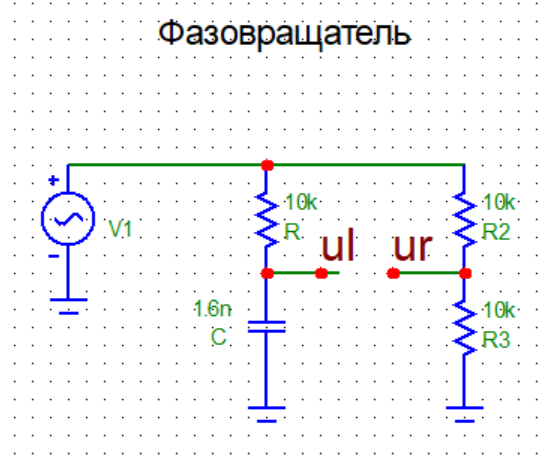
\includegraphics[scale=0.4]{phshift_omg.png}
\label{fig:Image1}
\end{figure} 

\begin{figure}[h!]
\centering
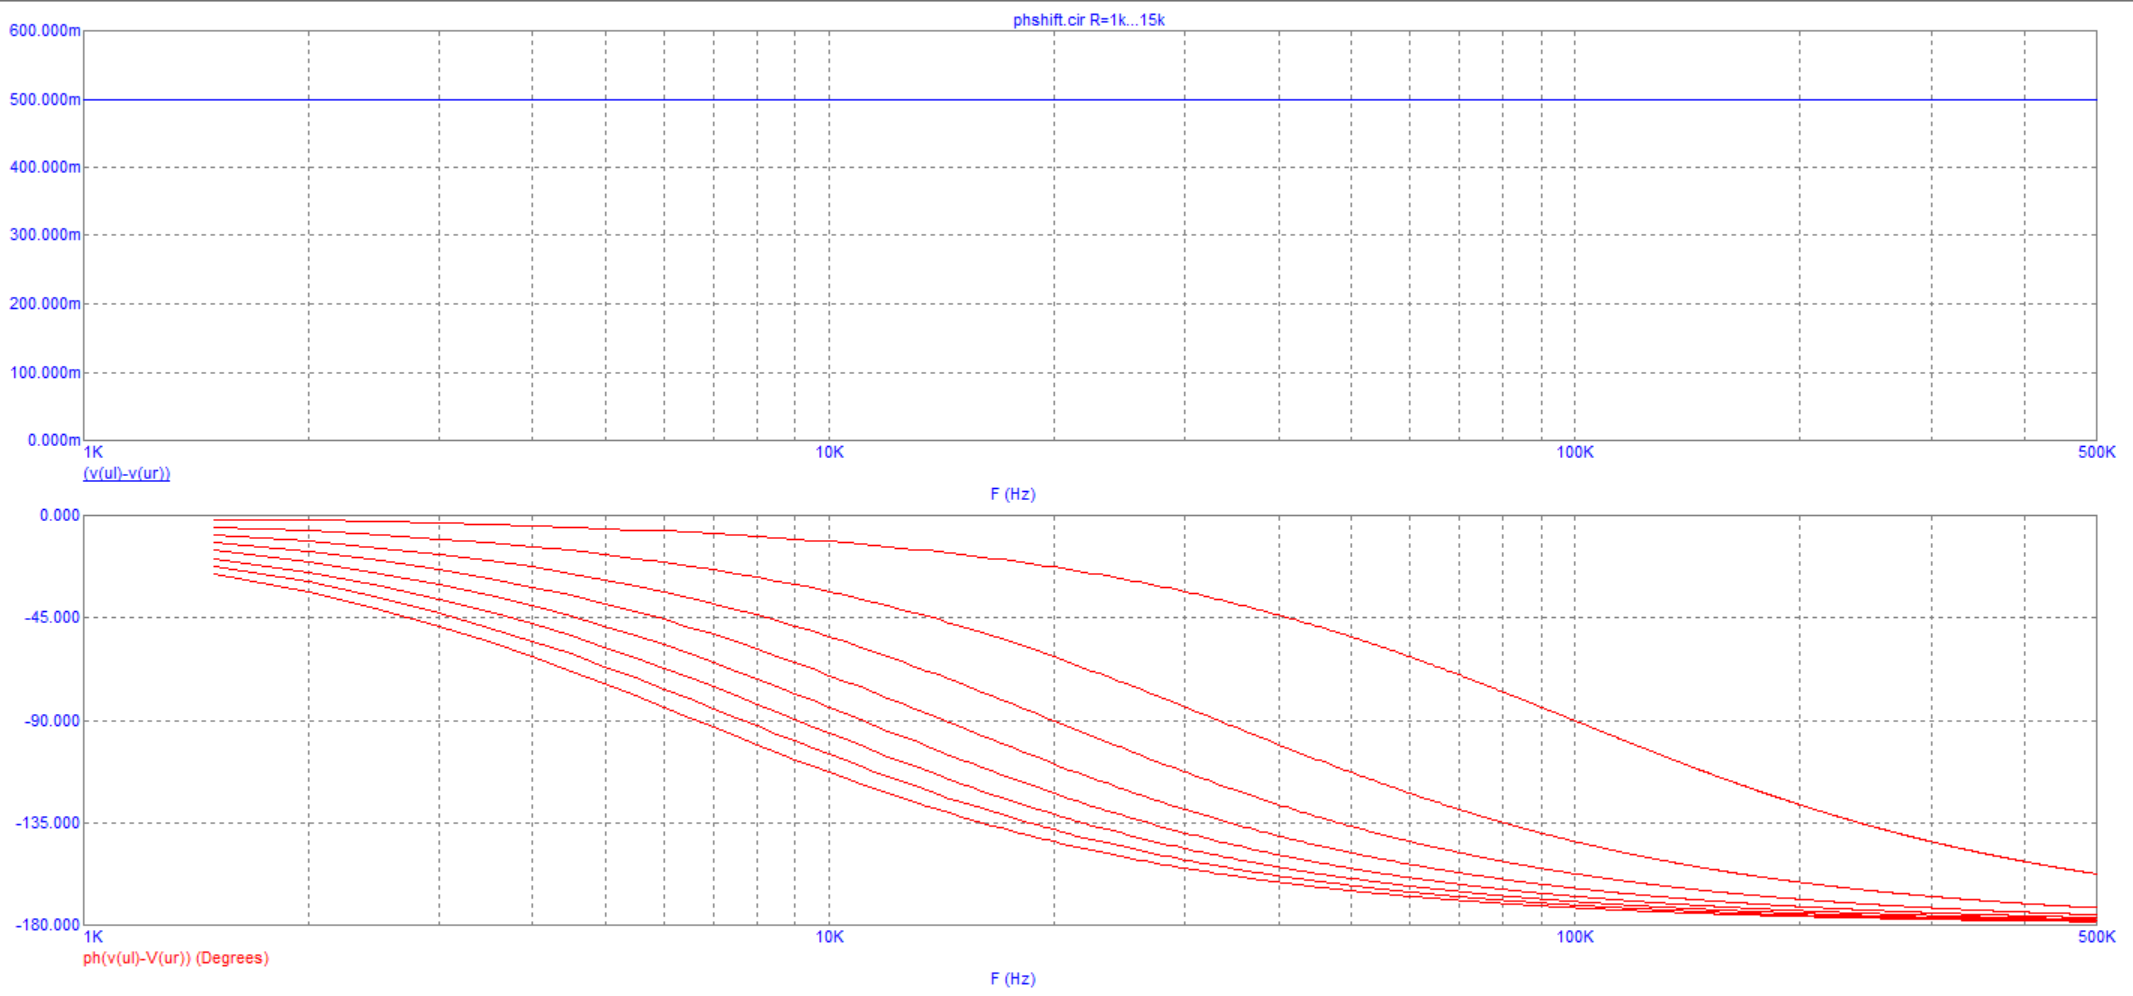
\includegraphics[scale=0.4]{phshift.png}
\label{fig:Image1}
\end{figure}

Наибольший диапазон перестройки реализуется на частоте $f = 20  \: \textit{кГц}$. Границы этого диапазона $[-143,4; -22,7]$.

\item Откроем модель двойного \textit{T}-моста \textbf{2tbridge.cir}.

\begin{figure}[h!]
\centering
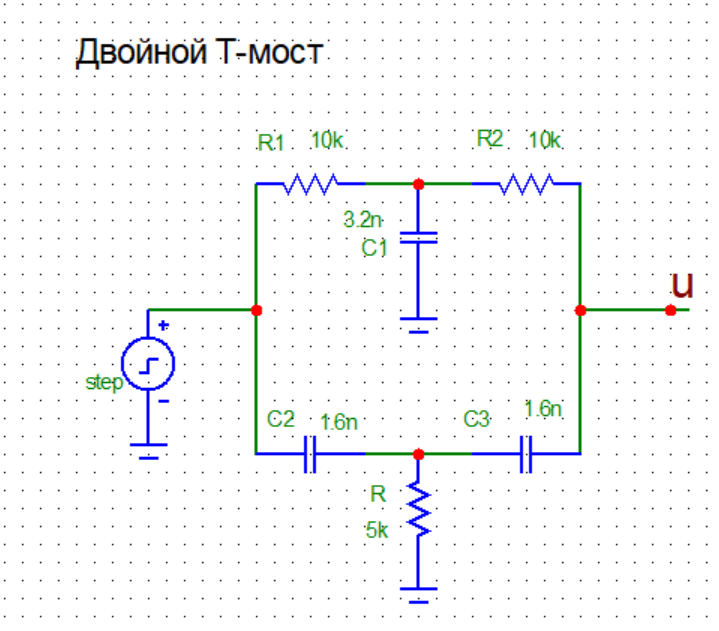
\includegraphics[scale=0.4]{2tbridge_img.png}
\label{fig:Image1}
\end{figure}

\begin{figure}[h!]
\centering
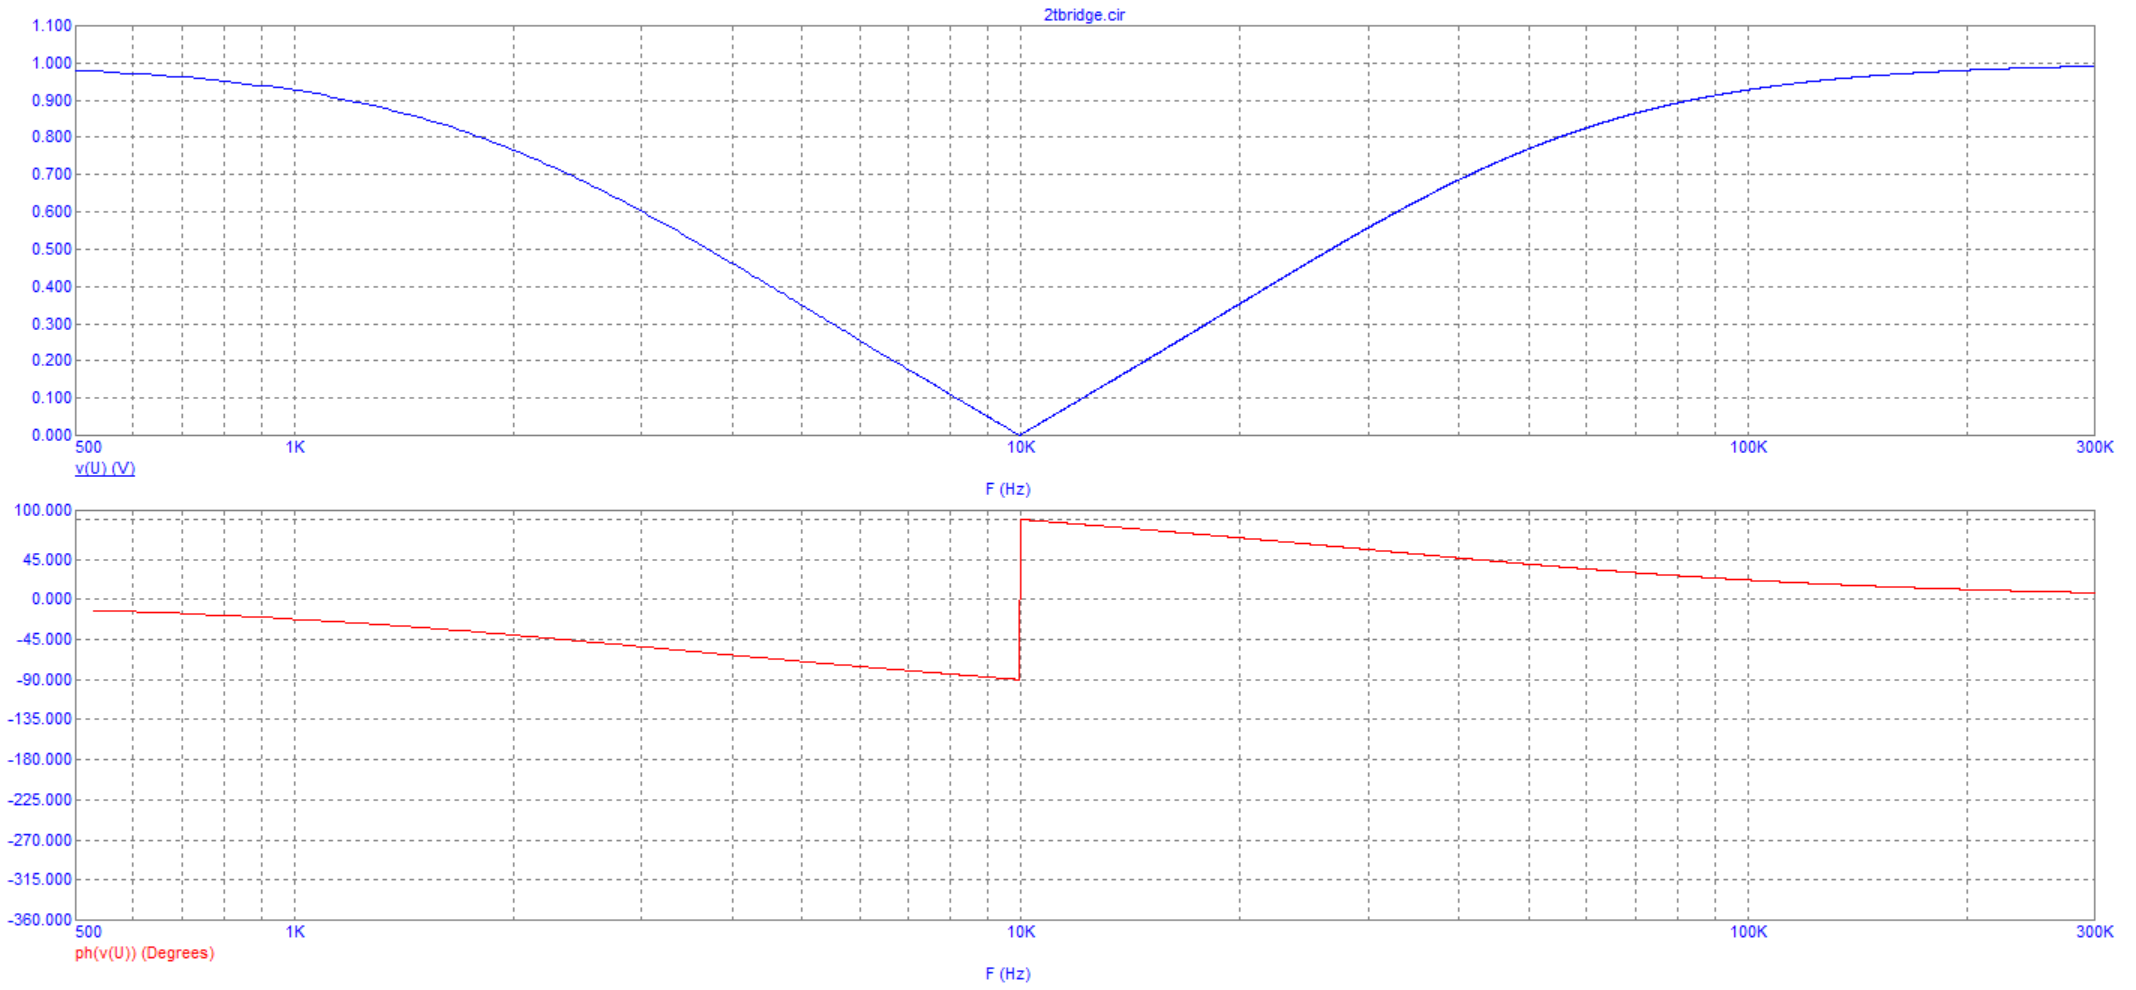
\includegraphics[scale=0.4]{2tbridge.png}
\label{fig:Image1}
\end{figure}

Измерим полосу режекции $\triangle f = 39 \: \textit{кГц}$. $f_0 = 10 \: \textit{кГц}$, следовательно выполняется $\triangle f = f_0$.

\begin{figure}[h!]
\centering
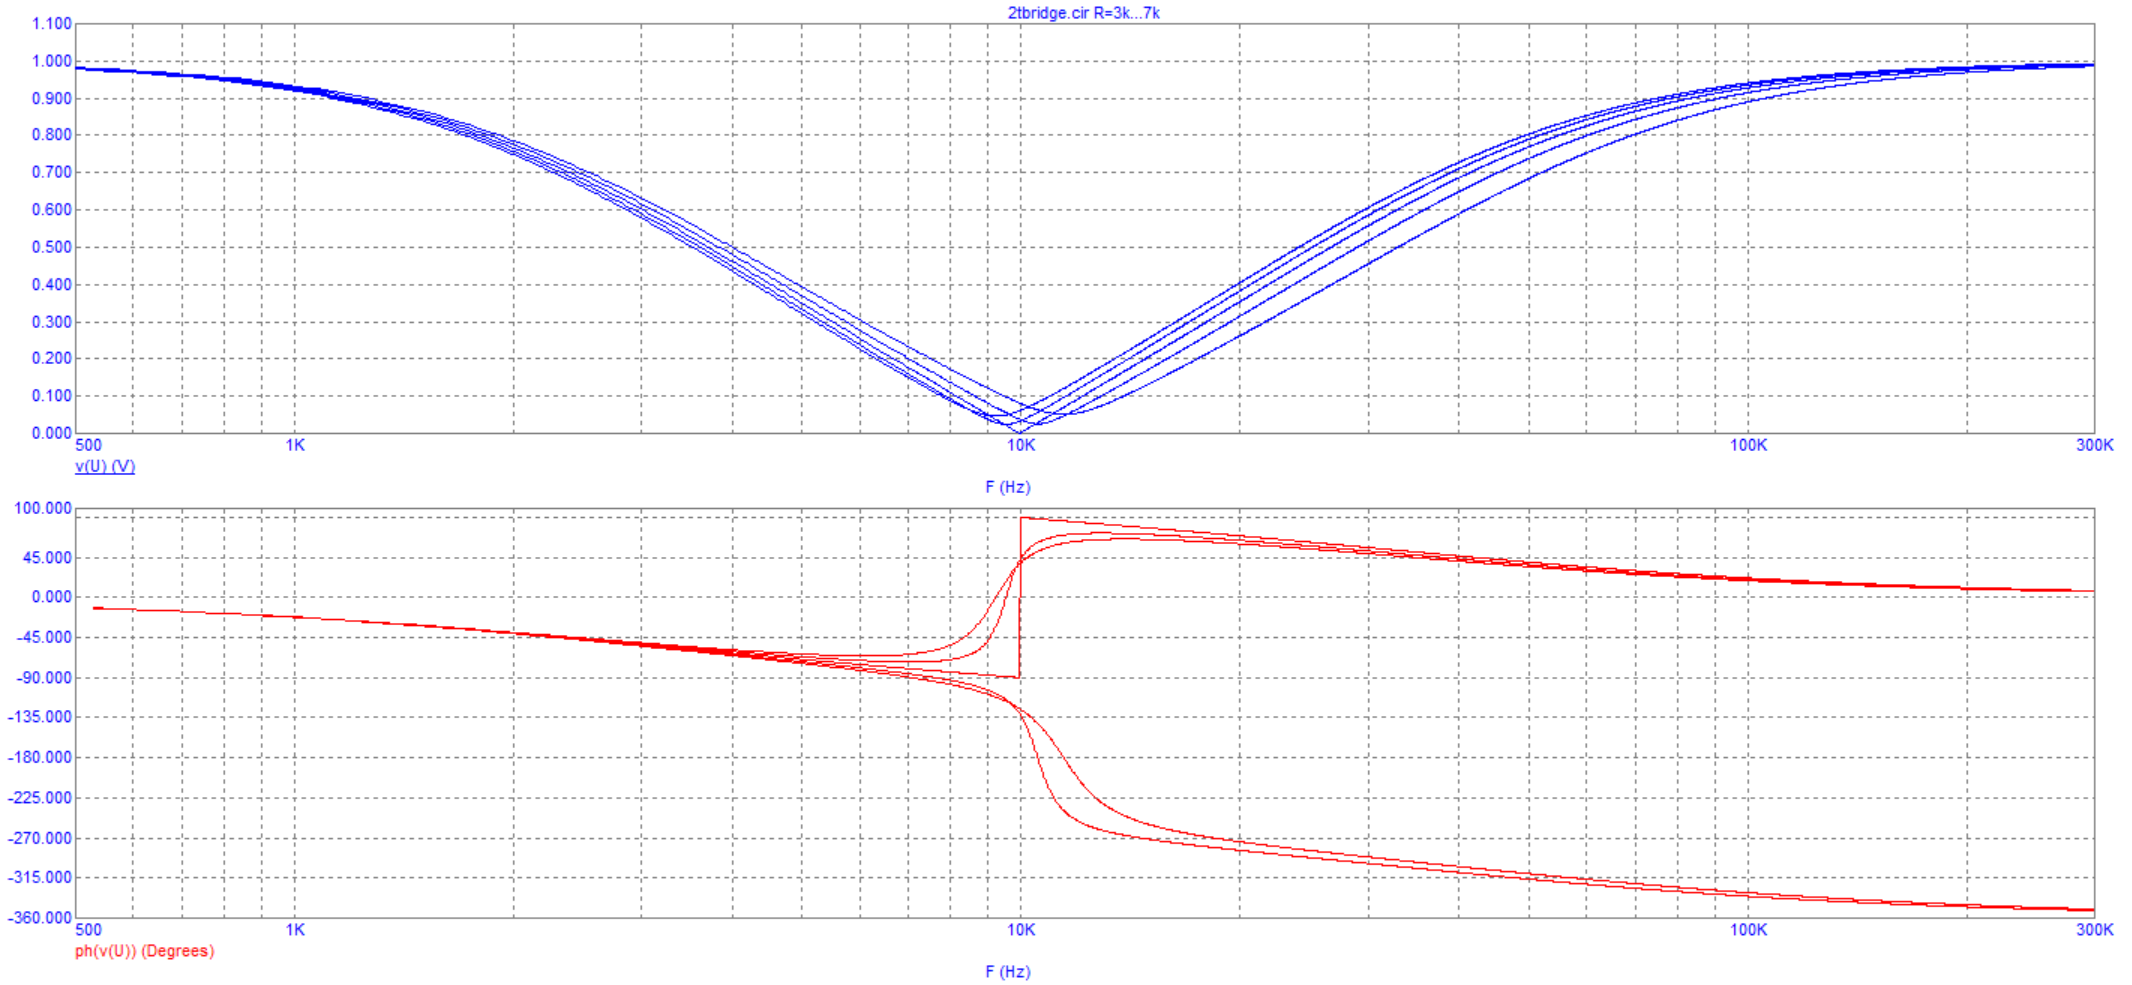
\includegraphics[scale=0.4]{2tbridge_AC2.png}
\label{fig:Image1}
\end{figure}

\begin{figure}[h!]
\centering
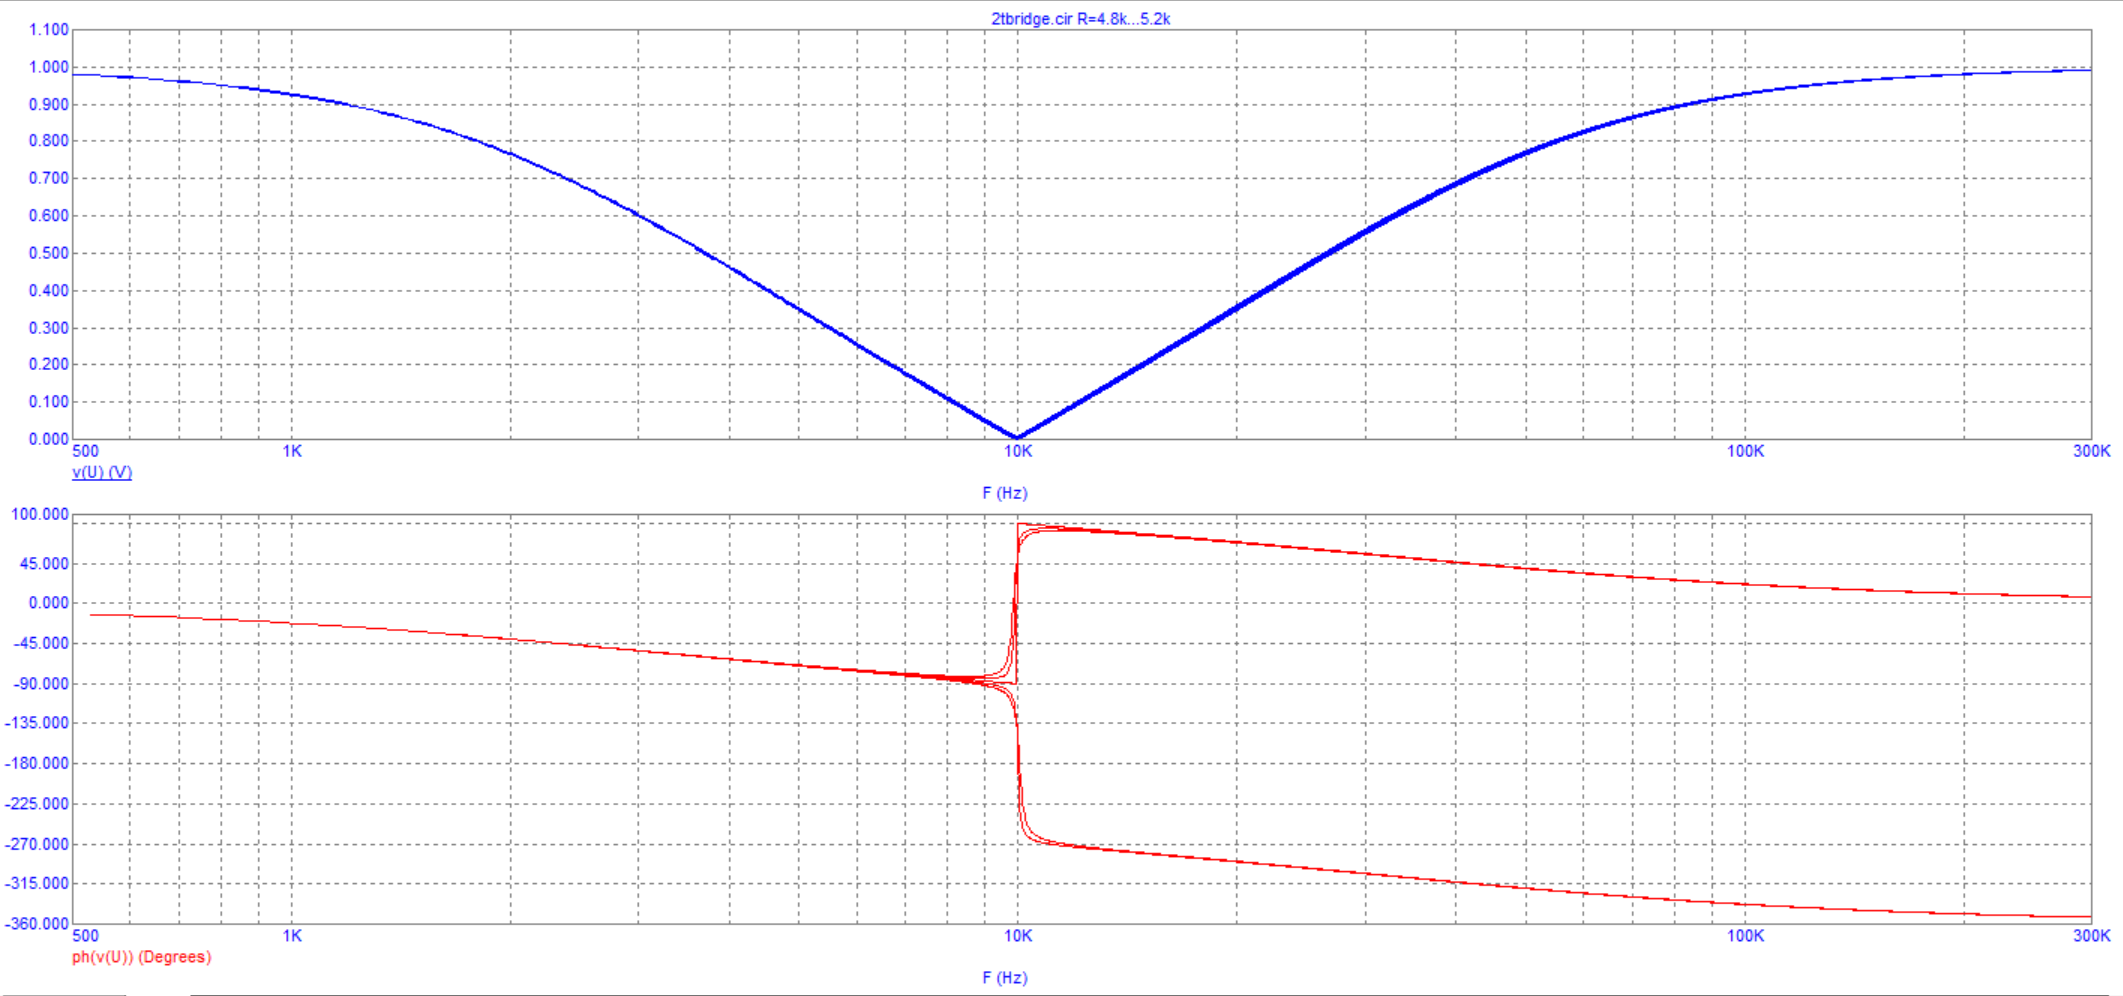
\includegraphics[scale=0.4]{2tbridge_AC3.png}
\label{fig:Image1}
\end{figure}

При росте $R$, $f_0$ падает. При $R = 5 \: \textit{кОм}$ наблюдается скачок на ФЧХ.

\item Подключив ко фходу источник прямоугольного импульса, проанализиурем переходную характеристику. $\tau_+ = 4 \: \textit{мкс}$, $\tau_- = 58 \: \textit{мкс}$. Это сходится с теоретическими значениями.

\begin{figure}[h!]
\centering
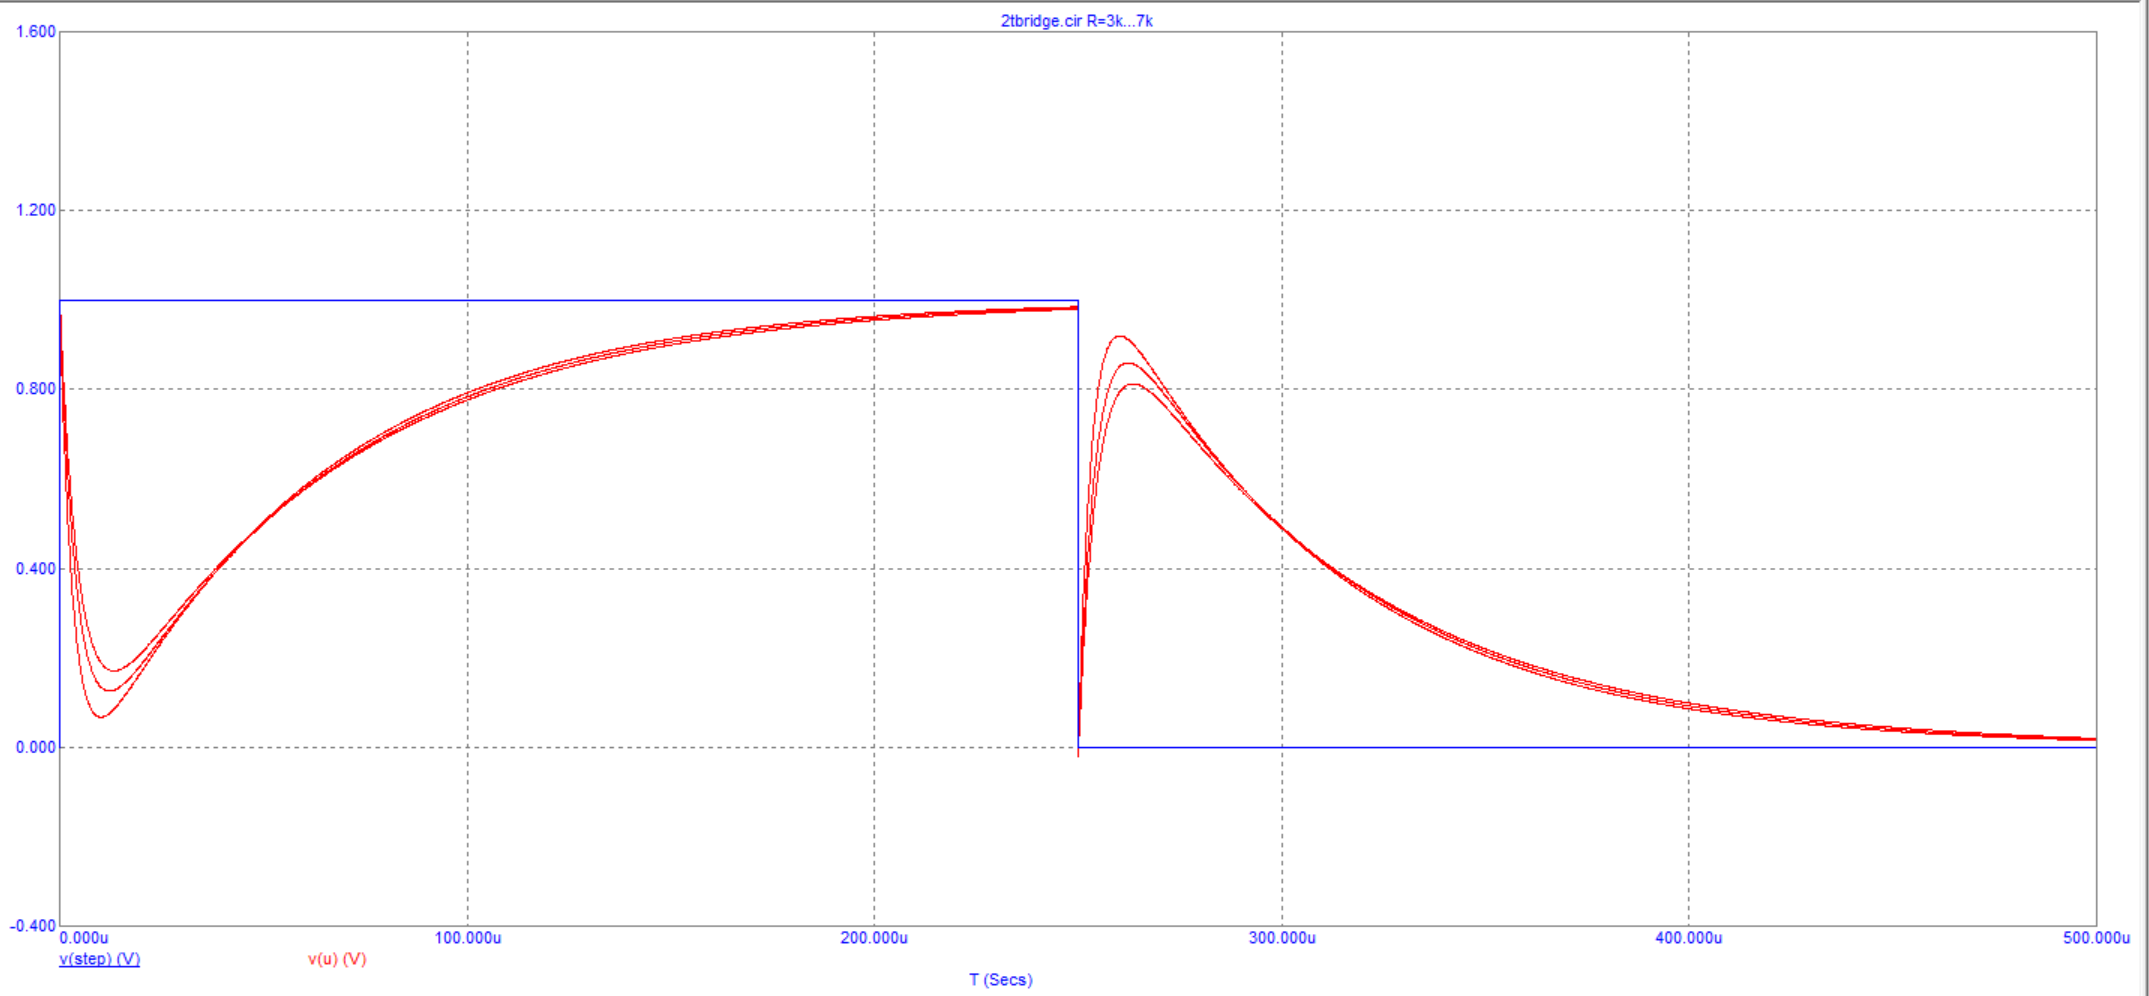
\includegraphics[scale=0.4]{2tbridge_AC4.png}
\label{fig:Image1}
\end{figure}

Варьирование приводит к усреднению функции.

\item Откроем модель \textbf{2tdelay.cir}. 

\begin{figure}[h!]
\centering
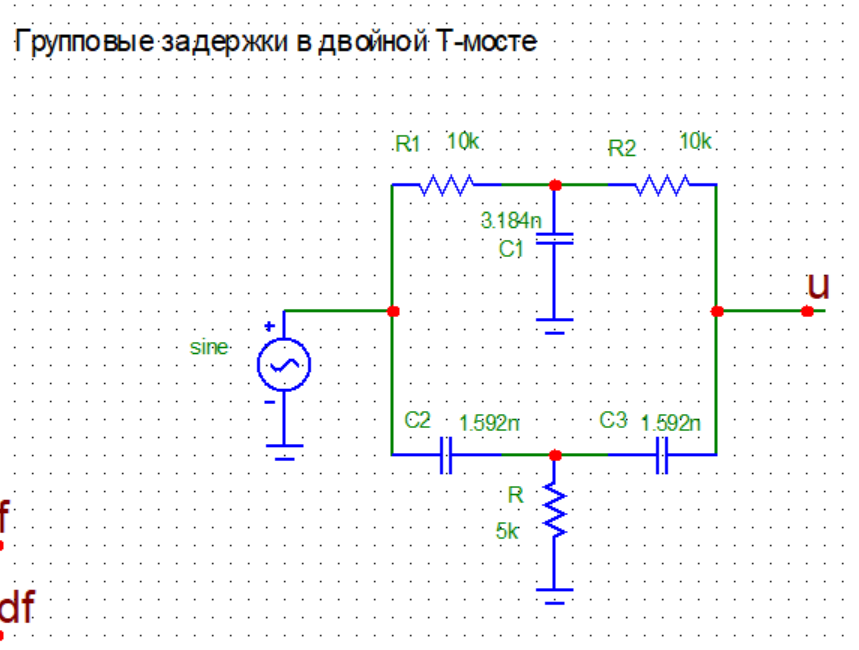
\includegraphics[scale=0.4]{2tdelay_img.png}
\label{fig:Image1}
\end{figure}

\begin{figure}[h!]
\centering
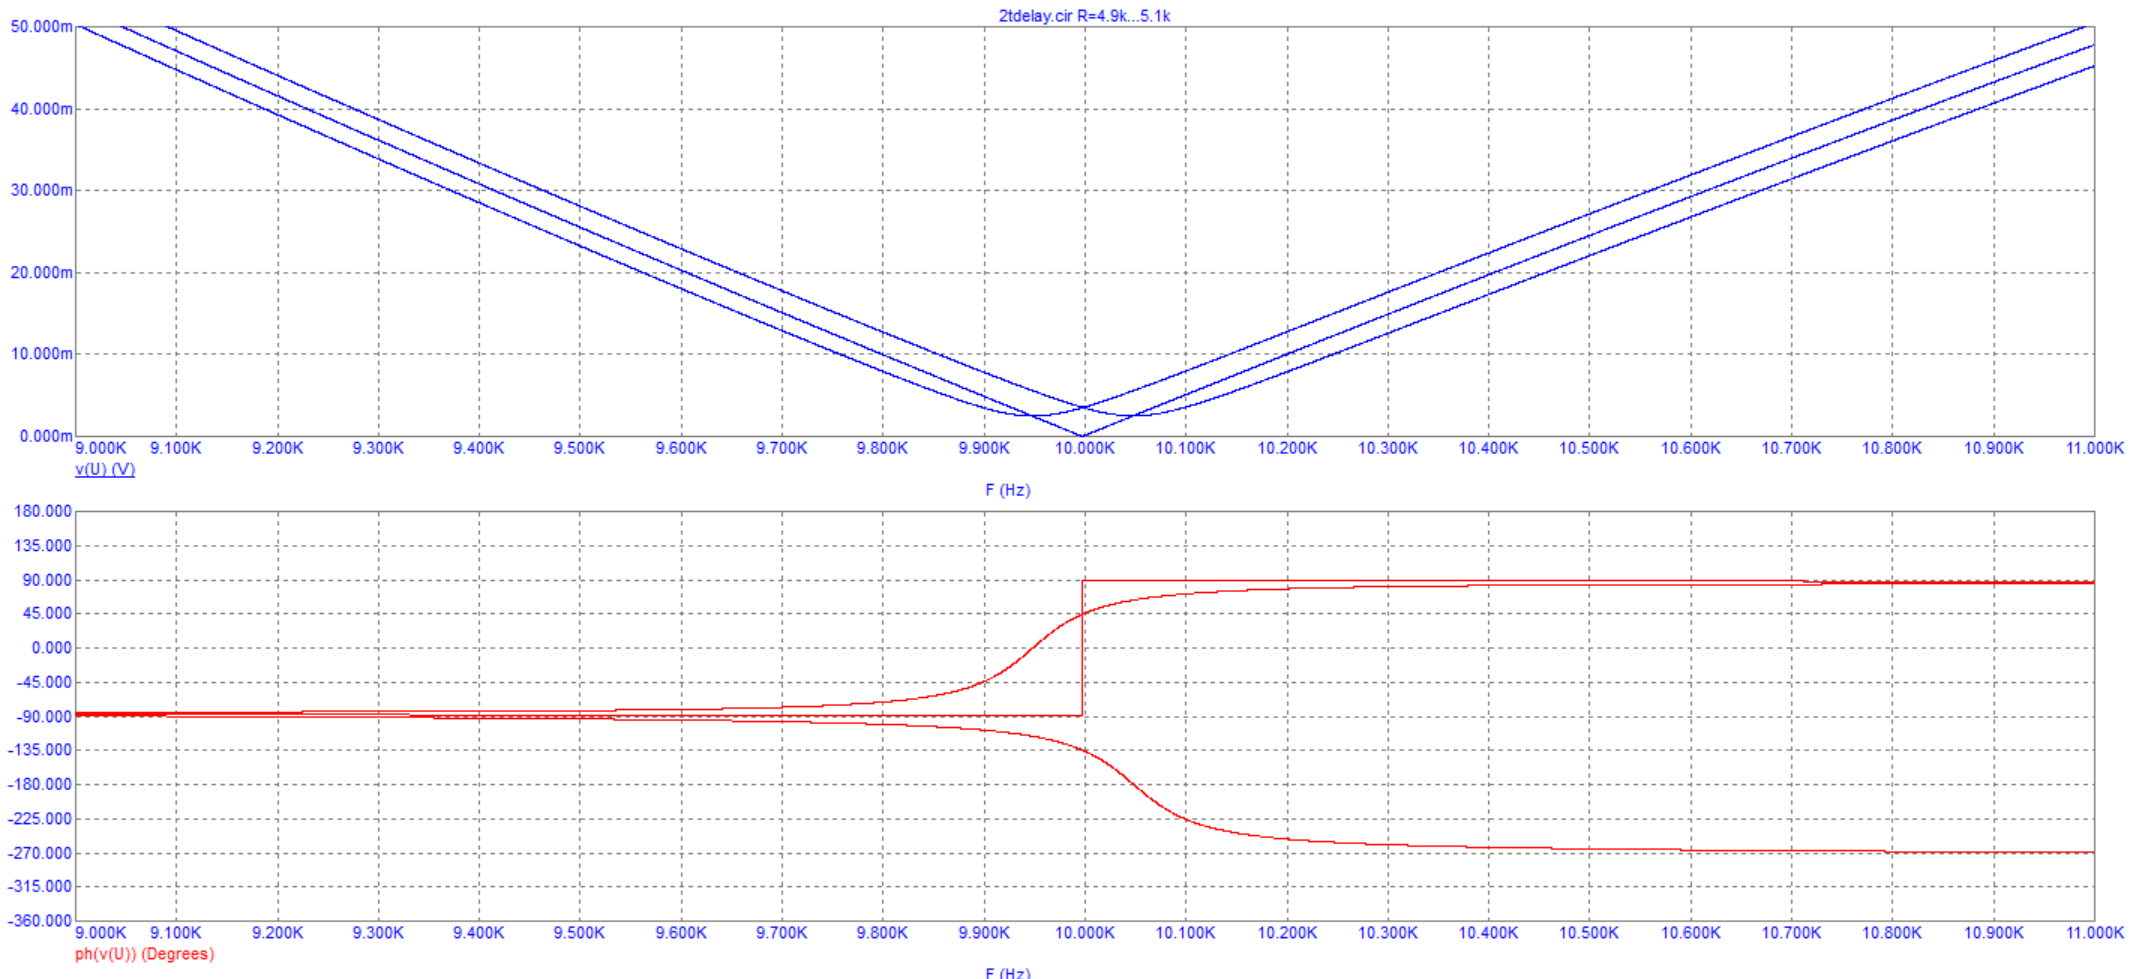
\includegraphics[scale=0.4]{2tdelay_AC1.png}
\label{fig:Image1}
\end{figure}

Оценим $Q = f_0/\triangle f$.

\begin{center}
\begin{tabular}{|c|c|c|c|}
\hline 
$R, \: \textit{кОм}$ & 4,9 & 5 & 5,1 \\ 
\hline 
$f_0, \: \textit{кГц}$ & 10,05 & 10 & 9,95 \\ 
\hline 
$\triangle f, \: \textit{кГц}$ & 0,05 & $10^{-4}\cdot 2,5$ & 0,05 \\ 
\hline 
$Q$ & 100,5 & 40000 & 99,5 \\ 
\hline 
\end{tabular}
\end{center}

В режиме \textit{Transient} измерим групповые задержки $\tau_g$:

\[\tau_g = 3 \: \textit{мс},\]

значение для обоих случаев ($R = 4,9 \: \textit{кОм}, f = 10,05 \: \textit{кГц}$ и $R = 5,1 \: \textit{кОм}, f = 9,95 \: \textit{кОм}$).

\begin{figure}[h!]
\centering
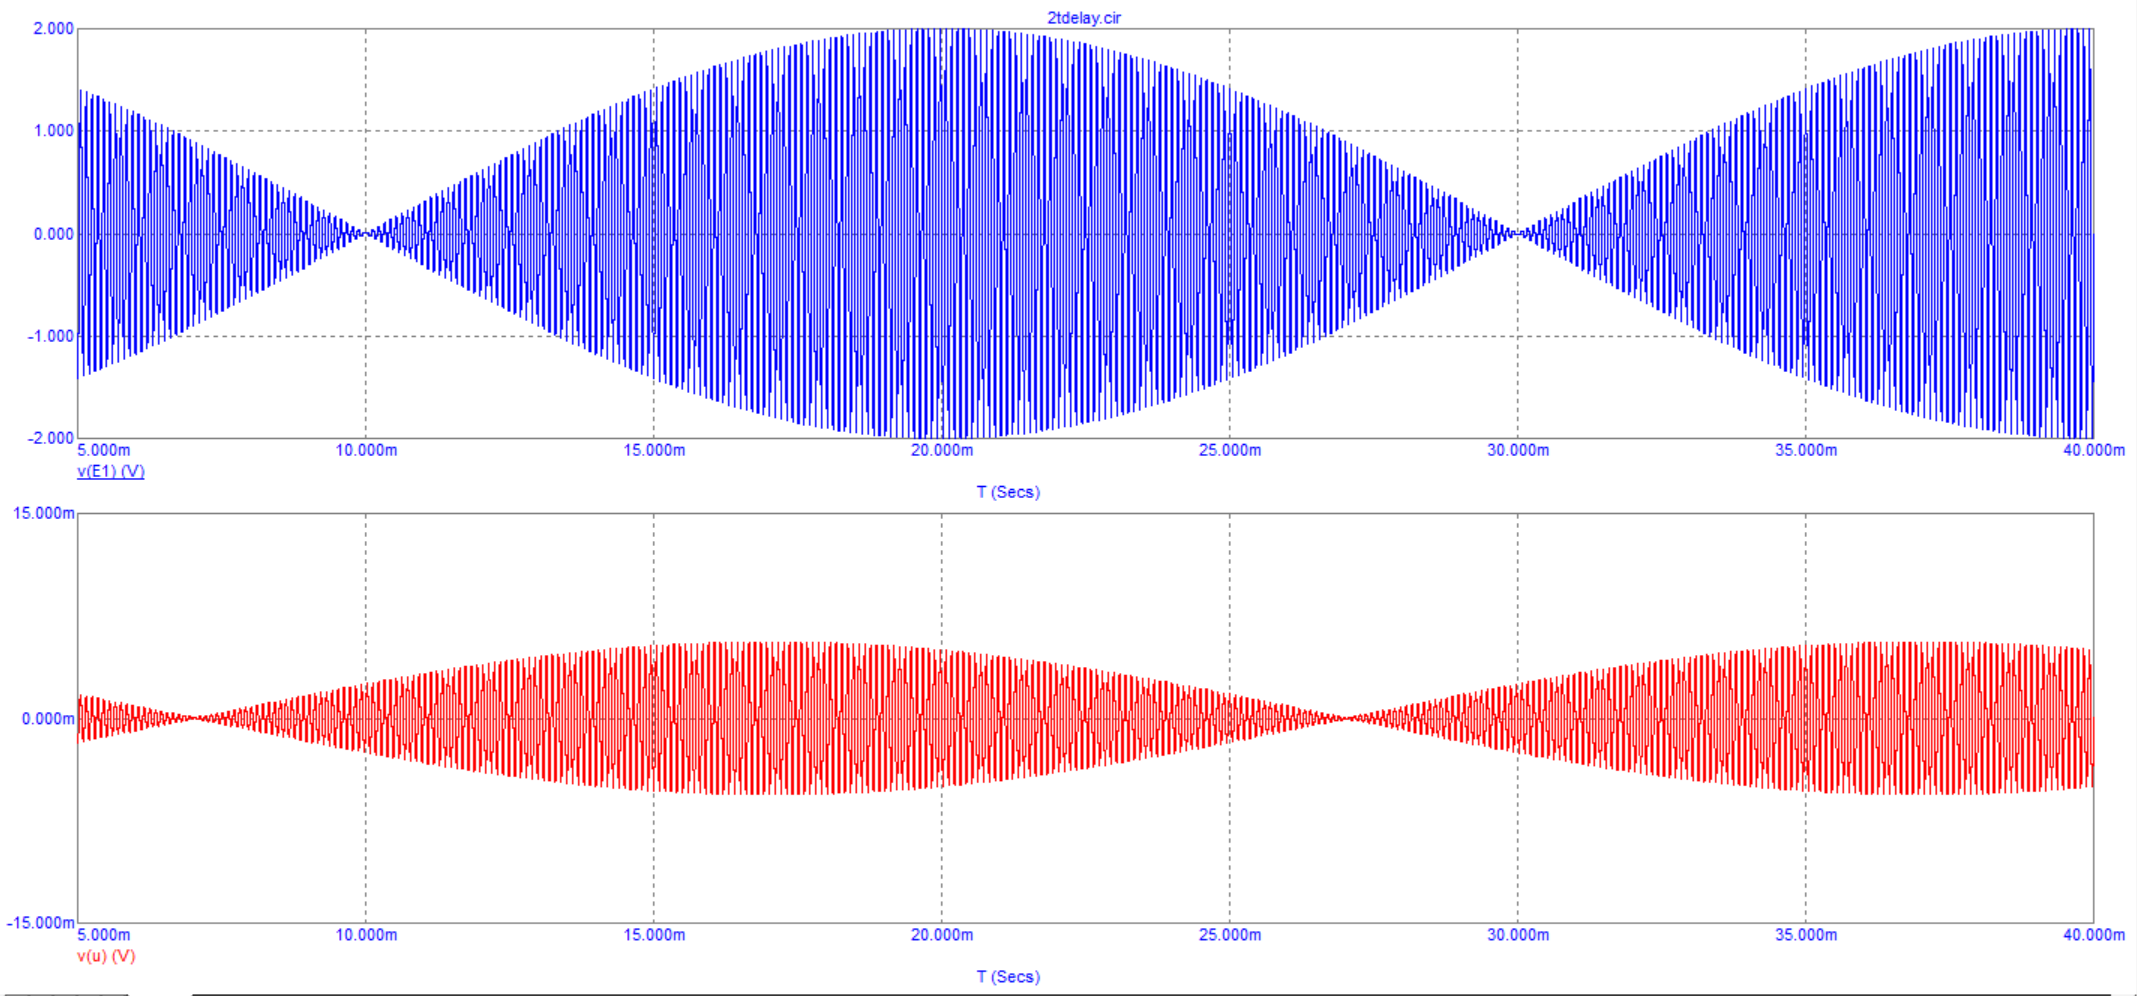
\includegraphics[scale=0.4]{2tdelay_AC2.png}
\label{fig:Image1}
\end{figure}

\end{enumerate}

\section*{ЗАДАНИЕ 4}

\begin{enumerate}

\item На макетной плате соберем схему полосового фильтра (его схема, как и схема ФНЧ и ФВЧ представлены на рисунке).

\begin{figure}[h!]
\centering
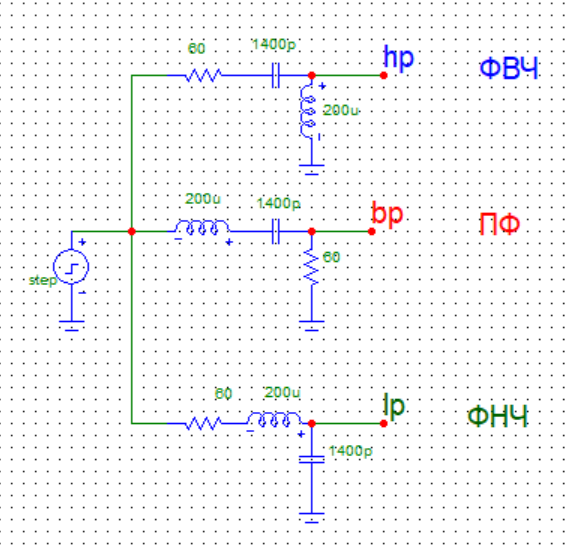
\includegraphics[scale=0.4]{rlc2pole_img.png}
\label{fig:Image1}
\end{figure}

\[L = 220 \: \textit{мкГн}\]
\[C = 1 \: \textit{мкФ}\]
\[r = 92 \: \textit{Ом}\]

Измерим резонансную частоту и коэффициент передачи:

\[f_0 = 366 \: \textit{кГц}\]

\[\triangle f = 75 \: \textit{кГц}\]

\[Q = \frac{f_0}{\triangle f} = 4,8\]

\item Из тех же компонент соберем схемы ФВЧ и ФНЧ. Измерим для них резонансную частоту и отношения $K(f_0)/K(0)$ для ФНЧ и $K(f_0)/K(\infty)$ для ФВЧ.

\[Q = \frac{K(f_0)}{K(0)} = 5,18\]

\[Q = \frac{K(f_0)}{K(\infty)} = 4,1\]

\item Подключим генератор прямоугольных импульсов. Изучим переходные характеристики ФВЧ, ФНЧ и ПФ. Прикинем по осцилограммам период колебаний и время их затухания до уровня $1/e = 0,37$ и дадим оценку резонансной частоты и добротности.

Для ФВЧ:

\[T = 2,8 \: \textit{мкс}\]

\[\tau = 0,45 \: \textit{мкс}\]

\[f_0 = 365 \: \textit{кГц}\]

\[Q = 6,2\]

Для ФНЧ:

\[T = 2,83 \: \textit{мкс}\]

\[\tau = 0,49 \: \textit{мкс}\]

\[f_0 = 352 \: \textit{кГц}\]

\[Q = 5,7\]

Для ФВЧ:

\[T = 2,84 \: \textit{мкс}\]

\[\tau = 0,51 \: \textit{мкс}\]

\[f_0 = 351 \: \textit{кГц}\]

\[Q = 5,6\]

\item Откроем в MicroCap модель \textbf{rlc2pole.cir}, изучим частотные фазовые и переходные характеристики фильтров.

\begin{figure}[h!]
\centering
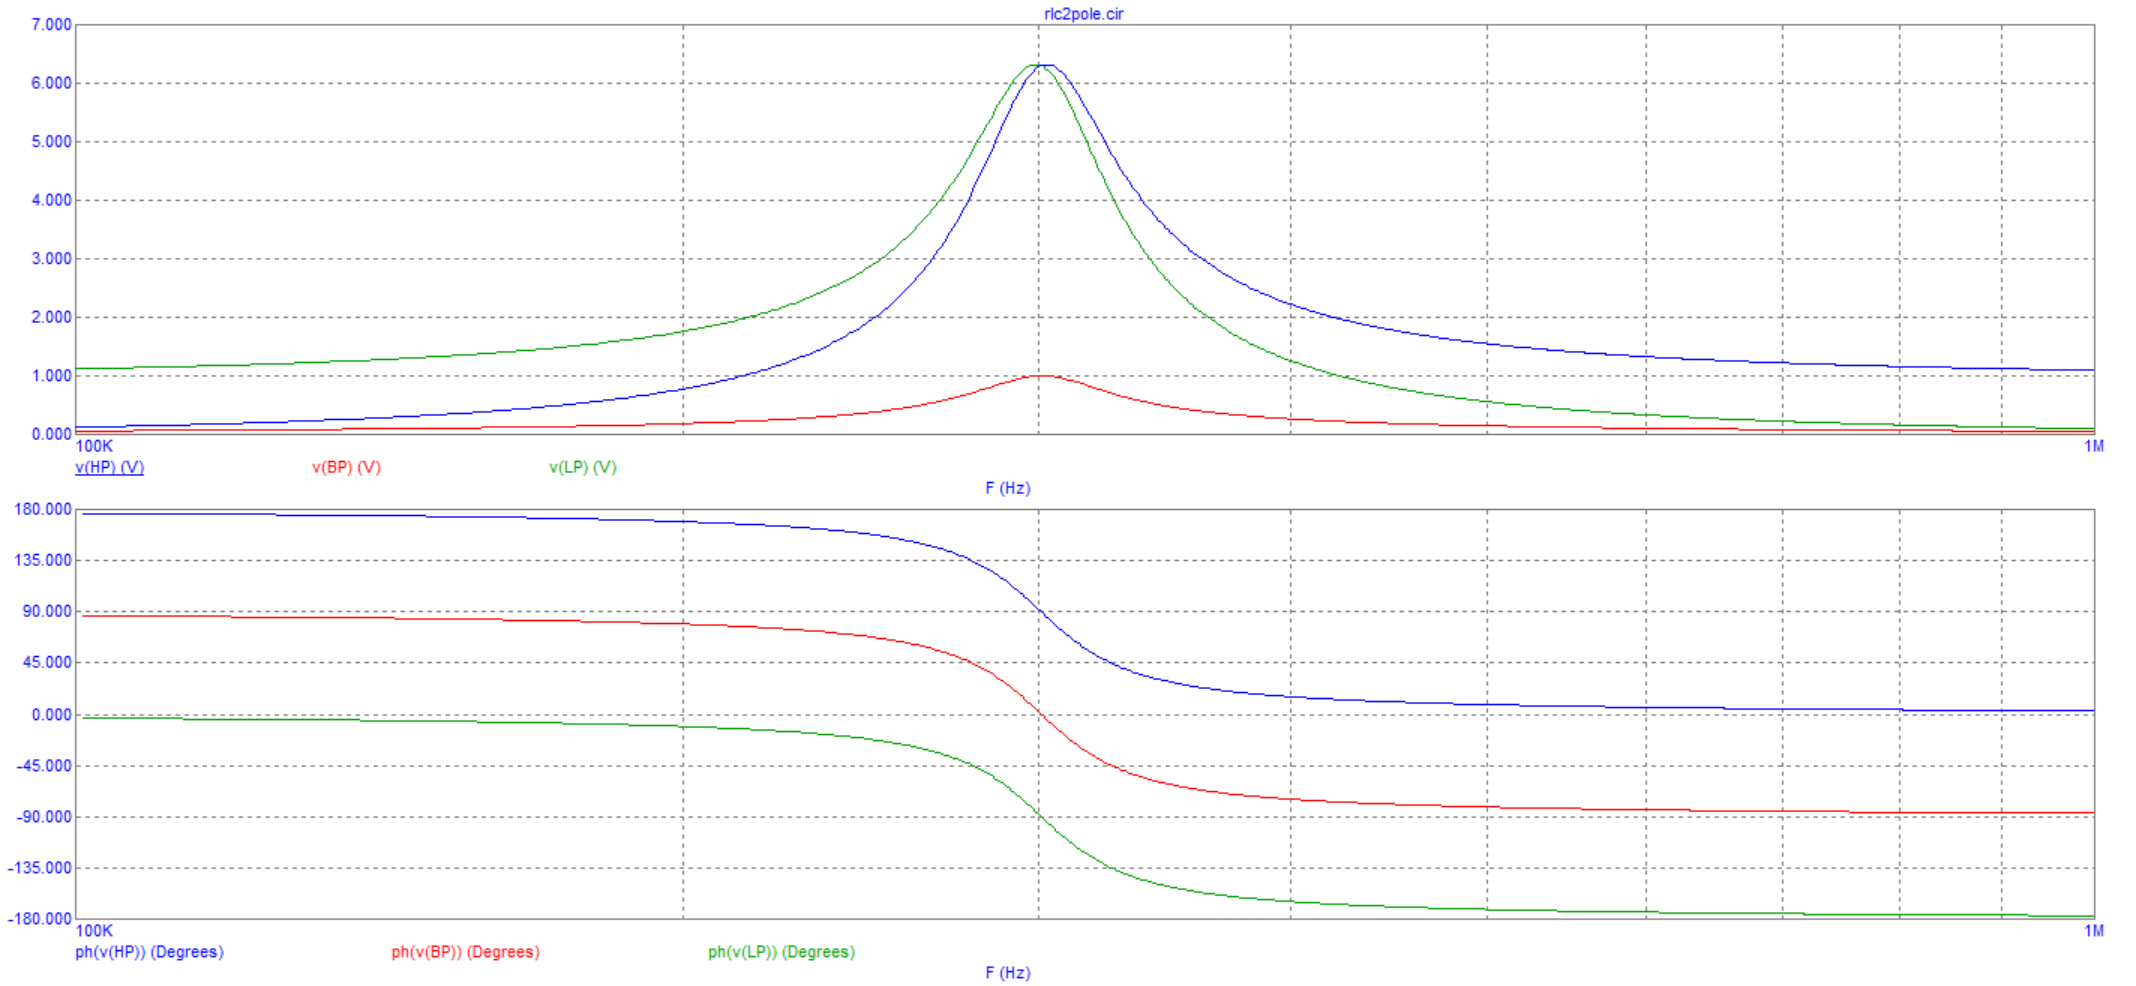
\includegraphics[scale=0.4]{rlc2pole_AC1.png}
\label{fig:Image1}
\caption{Частотные и фазовые характеристики}
\end{figure}

\begin{figure}[h!]
\centering
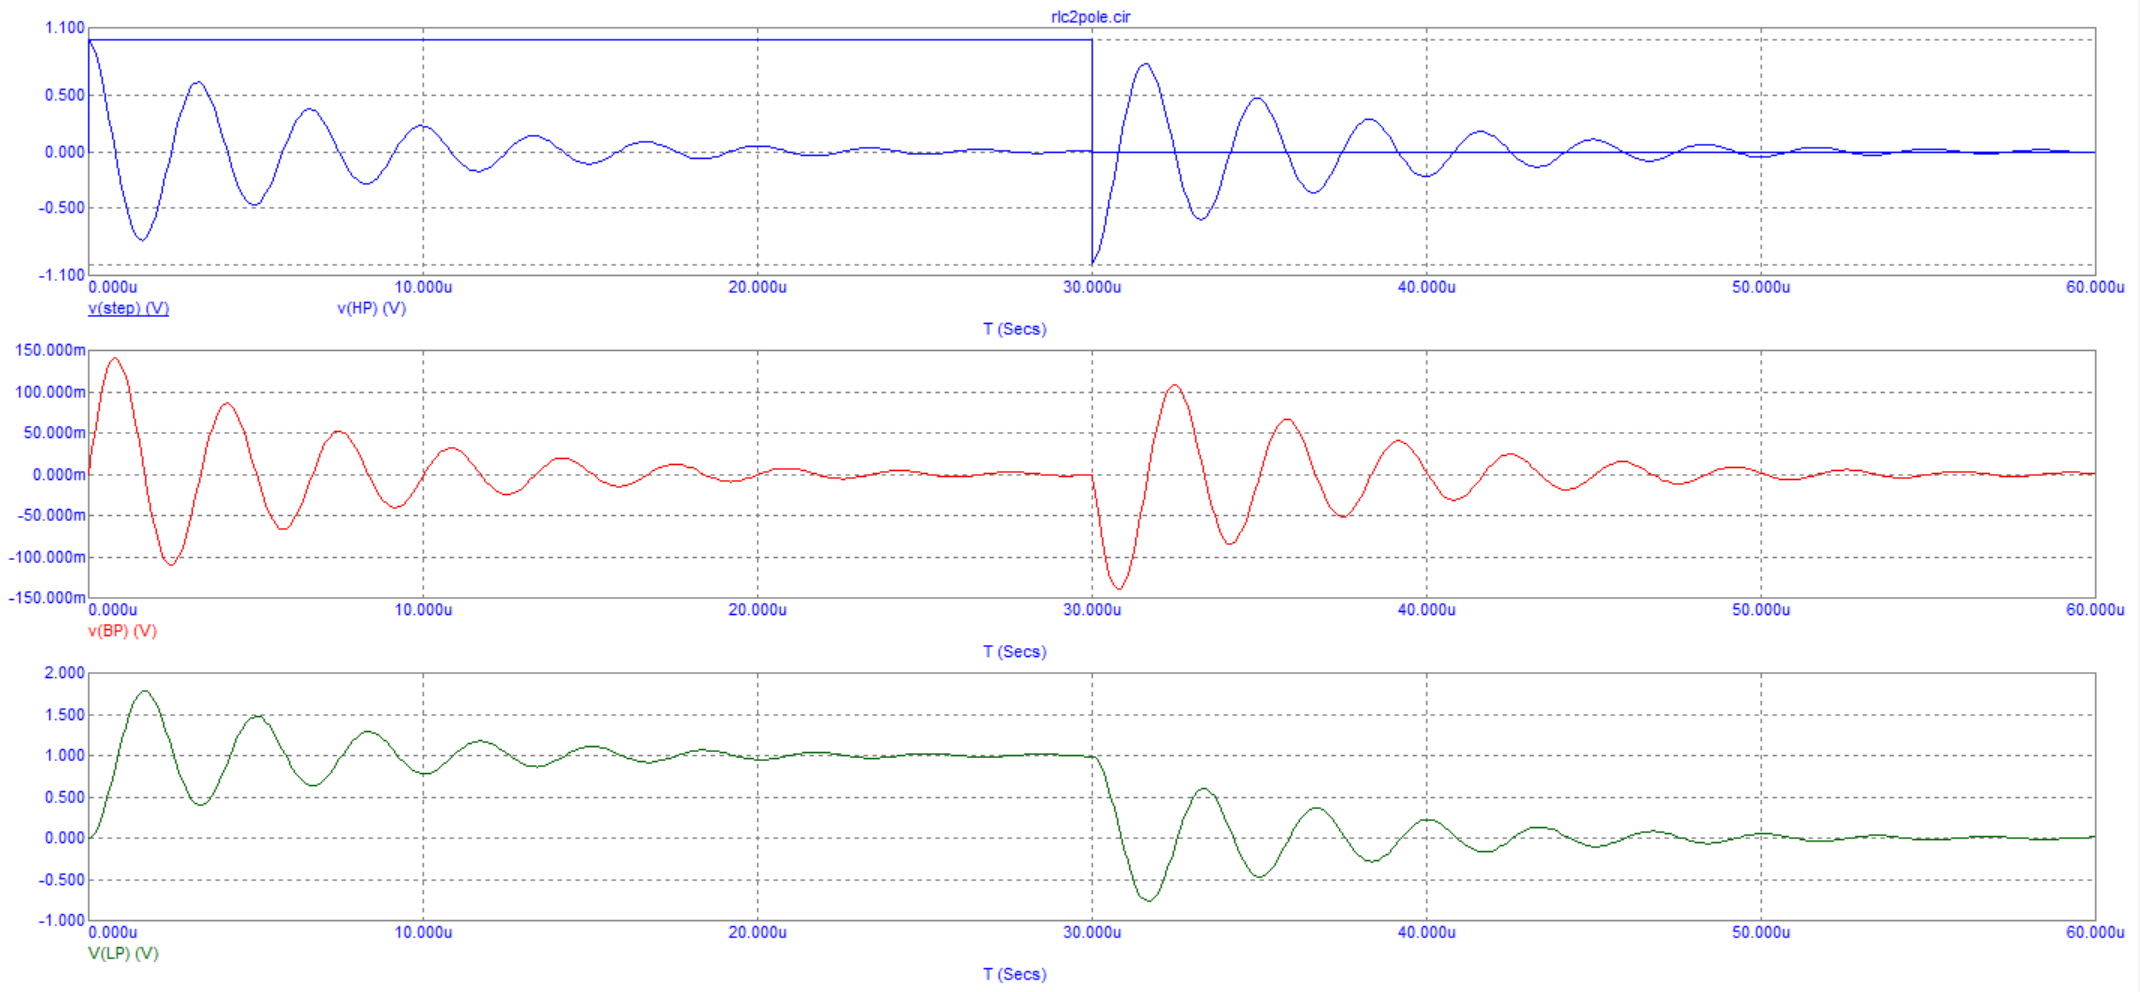
\includegraphics[scale=0.4]{rlc2pole_transient.png}
\label{fig:Image1}
\caption{Переходные характеристики}
\end{figure}

\item Откроем модель \textbf{groupdel.cir} полосового фильтра. Наблюдая в режиме \textit{Transient} отклик на двухчастотный сигнал изучим зависимость групповой задержки $\tau_g$ от $R = 10, 20, 40, 100$.

\begin{center}
\begin{tabular}{|c|c|c|c|c|}
\hline 
$R, \: \textit{Ом}$ & 10 & 20 & 40 & 100 \\ 
\hline 
$\tau_g, \: \textit{мс}$ & 0,5 & 0,29 & 0,152 & 0,064 \\ 
\hline 
$\tau_{\textit{теор}}, \: \textit{мс}$ & 0,62 & 0,31 & 0,155 & 0,06 \\ 
\hline 
Q & 195 & 98 & 49 & 19 \\ 
\hline 
\end{tabular}
\end{center}

\item Откроем модель \textbf{lcpower.cir}.

\begin{figure}[h!]
\centering
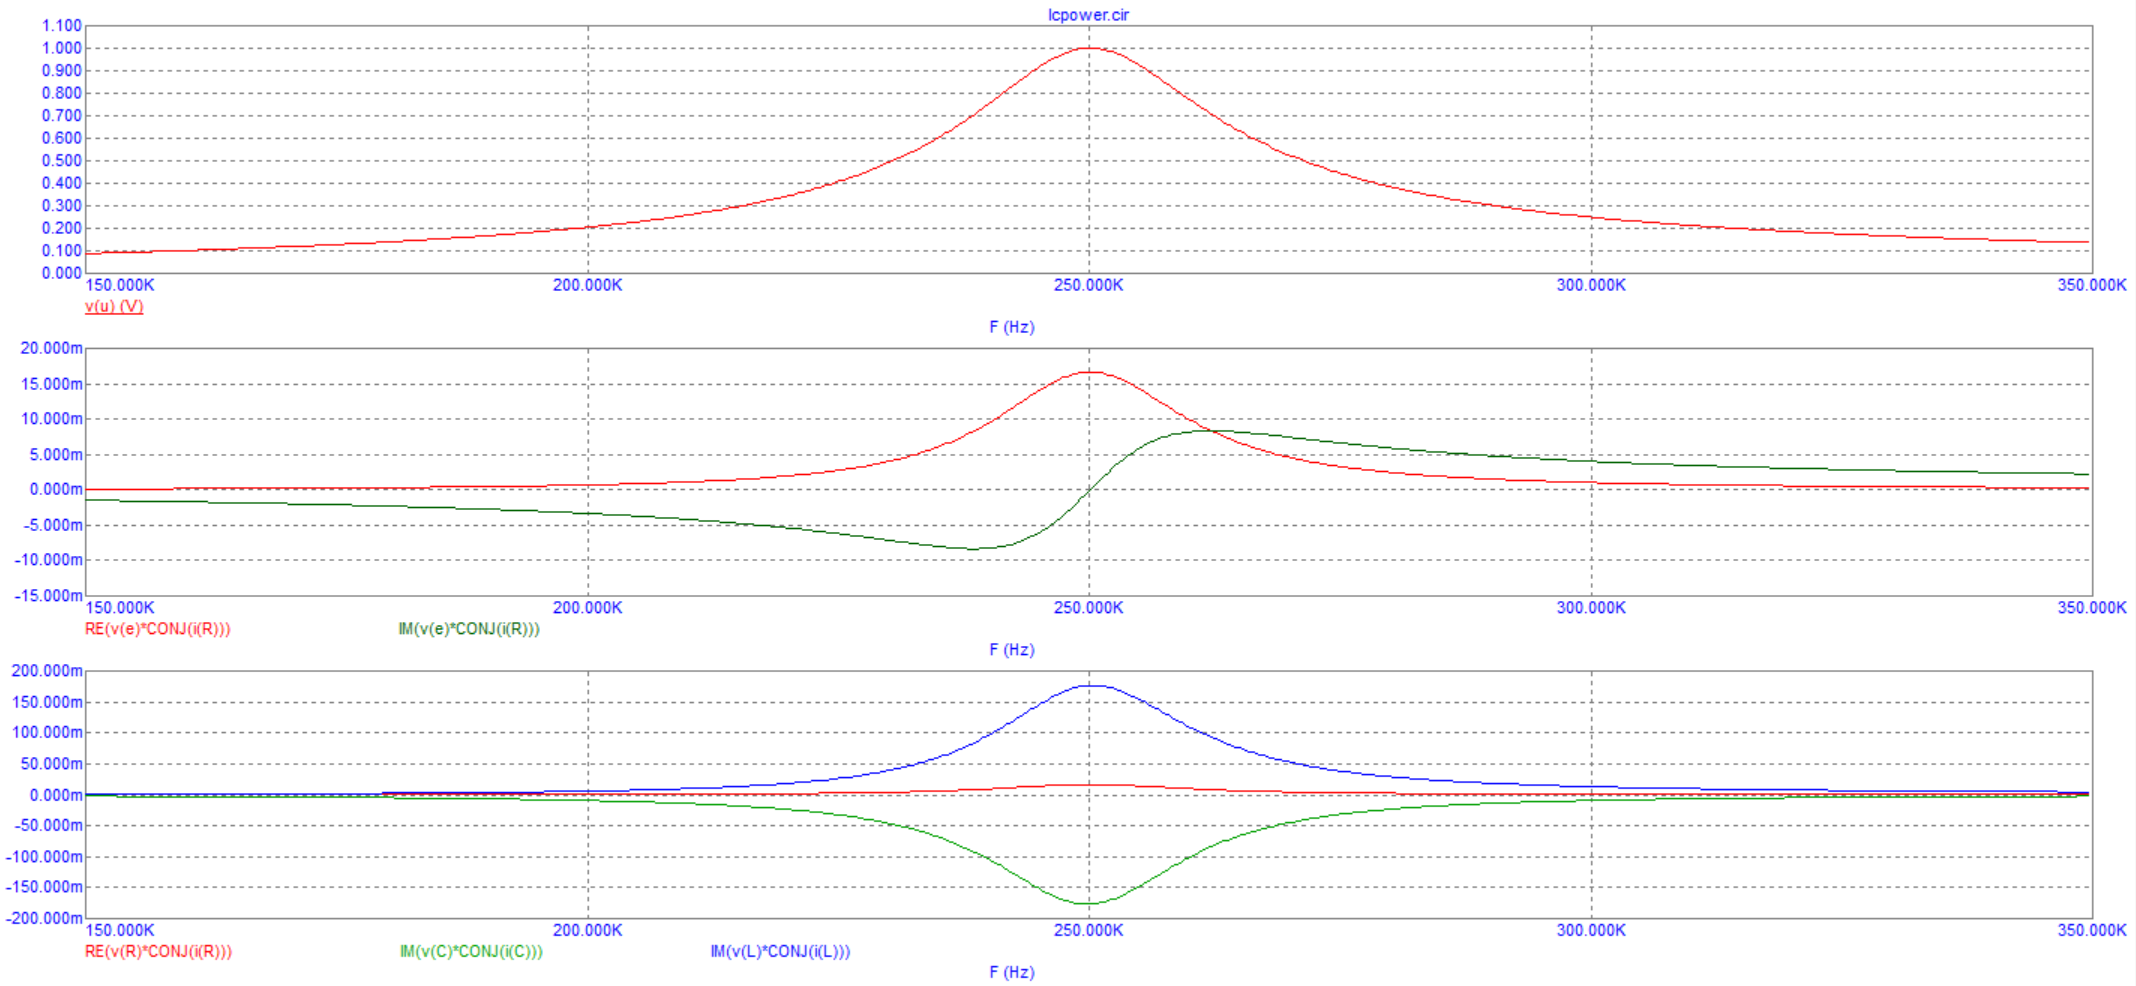
\includegraphics[scale=0.4]{lcpower.png}
\label{fig:Image1}
\end{figure} 

На частоте резонанса $f_0 = 250 \: \textit{кГц}$.

\[P_L = 176,066 \: m \quad P_C = -177,477 \: m \quad P_R = 15,89 \: m \Rightarrow \sum P = 14,47\]

\[P_{\sum \textit{теор}} = 16,18 \: m\]

На одной из границ полосы пропускания $f_1 = 238 \: \textit{кГц}$:

\[P_L = 116,577 \: m \quad P_C = -122,51 \: m \quad P_R = 11,14 \: m \Rightarrow \sum P = 5,147\]

\[P_{\sum \textit{теор}} = 11,367 \: m\]

Закон суммирования выполняется.

\end{enumerate}

\section*{ЗАДАНИЕ 5}

\begin{enumerate}

\item Откроем в MicroCap модель \textbf{parallel.cir} параллельного контура с $f_0 = 100 \: \textit{кГц}$, $\varrho = 570$. По схеме оценим параметры:

\[\alpha = \frac{\rho}{R_0}\]

\[\beta = \frac{R}{\rho}\]

\[Q = \frac{1}{\alpha + \beta}\]

\begin{figure}[h!]
\centering
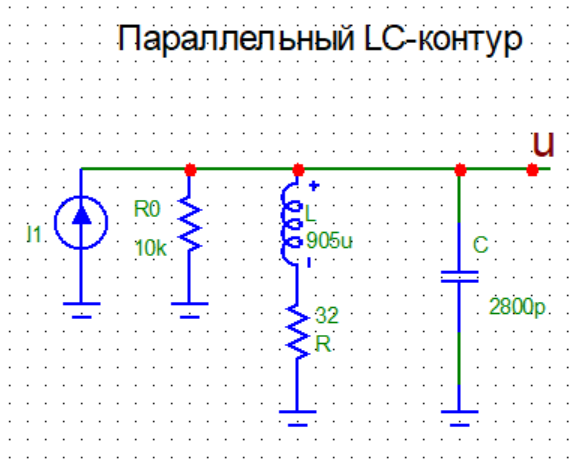
\includegraphics[scale=0.4]{parallel_img.png}
\label{fig:Image1}
\end{figure} 

\[\rho = \sqrt{\frac{L}{C}} = 568\]

\[\alpha = 0,0568 \quad \beta = 0,0563\]

\[Q = 8,84\]

\item Найдем резонансную частоту $f_0 = 100 \: \textit{кГц}$, полосу пропускания $\triangle f = 11,6 \: \textit{кГц}$. Измерим сопротивление контура $R_0 = 5 \: \textit{кОм}$. Оценим добротность как:

\[Q = \frac{R_0}{\rho} = 8,8\]

\[Q = \frac{f_0}{\triangle f} = 8,6\]

\item Изучим влияние на добротность последовательных потерь \textit{R}, установив варьирование $R = [0, 32 \Vert 32]$. 

\begin{figure}[h!]
\centering
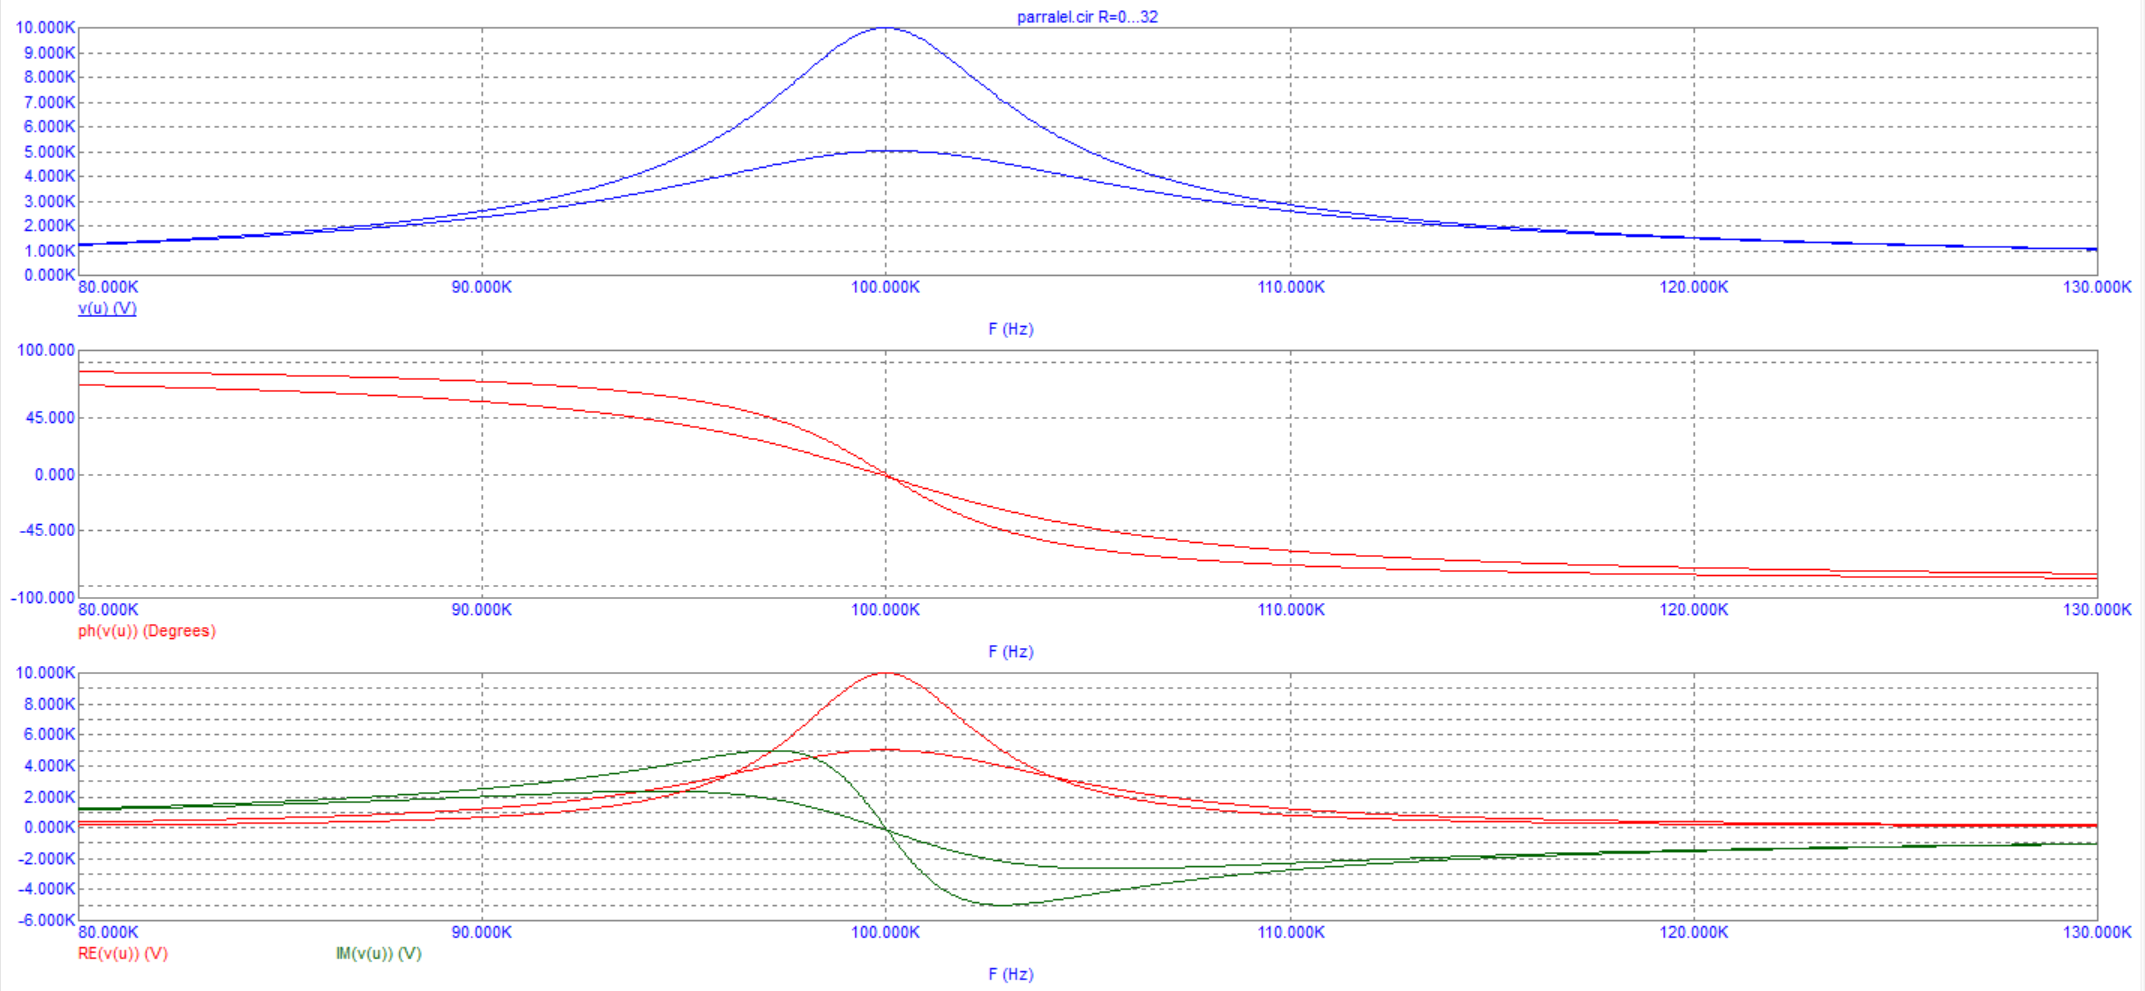
\includegraphics[scale=0.4]{parallel_AC1.png}
\label{fig:Image1}
\end{figure} 

Добротность при $R = 0$:

\[Q = \frac{f_0}{\triangle f} = 17,3\]

Изучим влияние параллельных потерь $R_0$, установив варьирование $R_0 = [10k, 1000k \Vert 1000k]$. Измерим добротность при $R_0 = 1000 \: \textit{кОм}$:

\[Q = \frac{f_0}{\triangle f} = 17,2\]

При увеличении $R$ от 0 \textit{Ом} до 32 \textit{Ом} $1/Q$ меняется от 0,058 до 0,116. При увеличении $R_0$ от 10 \textit{кОм} до 1000 \textit{кОм} $1/Q$ меняется от 0,116 до 0,058.

\item Изучим зависимость частоты параллельного резонанса от $R = [0, 150 \Vert 50]$.

\begin{figure}[h!]
\centering
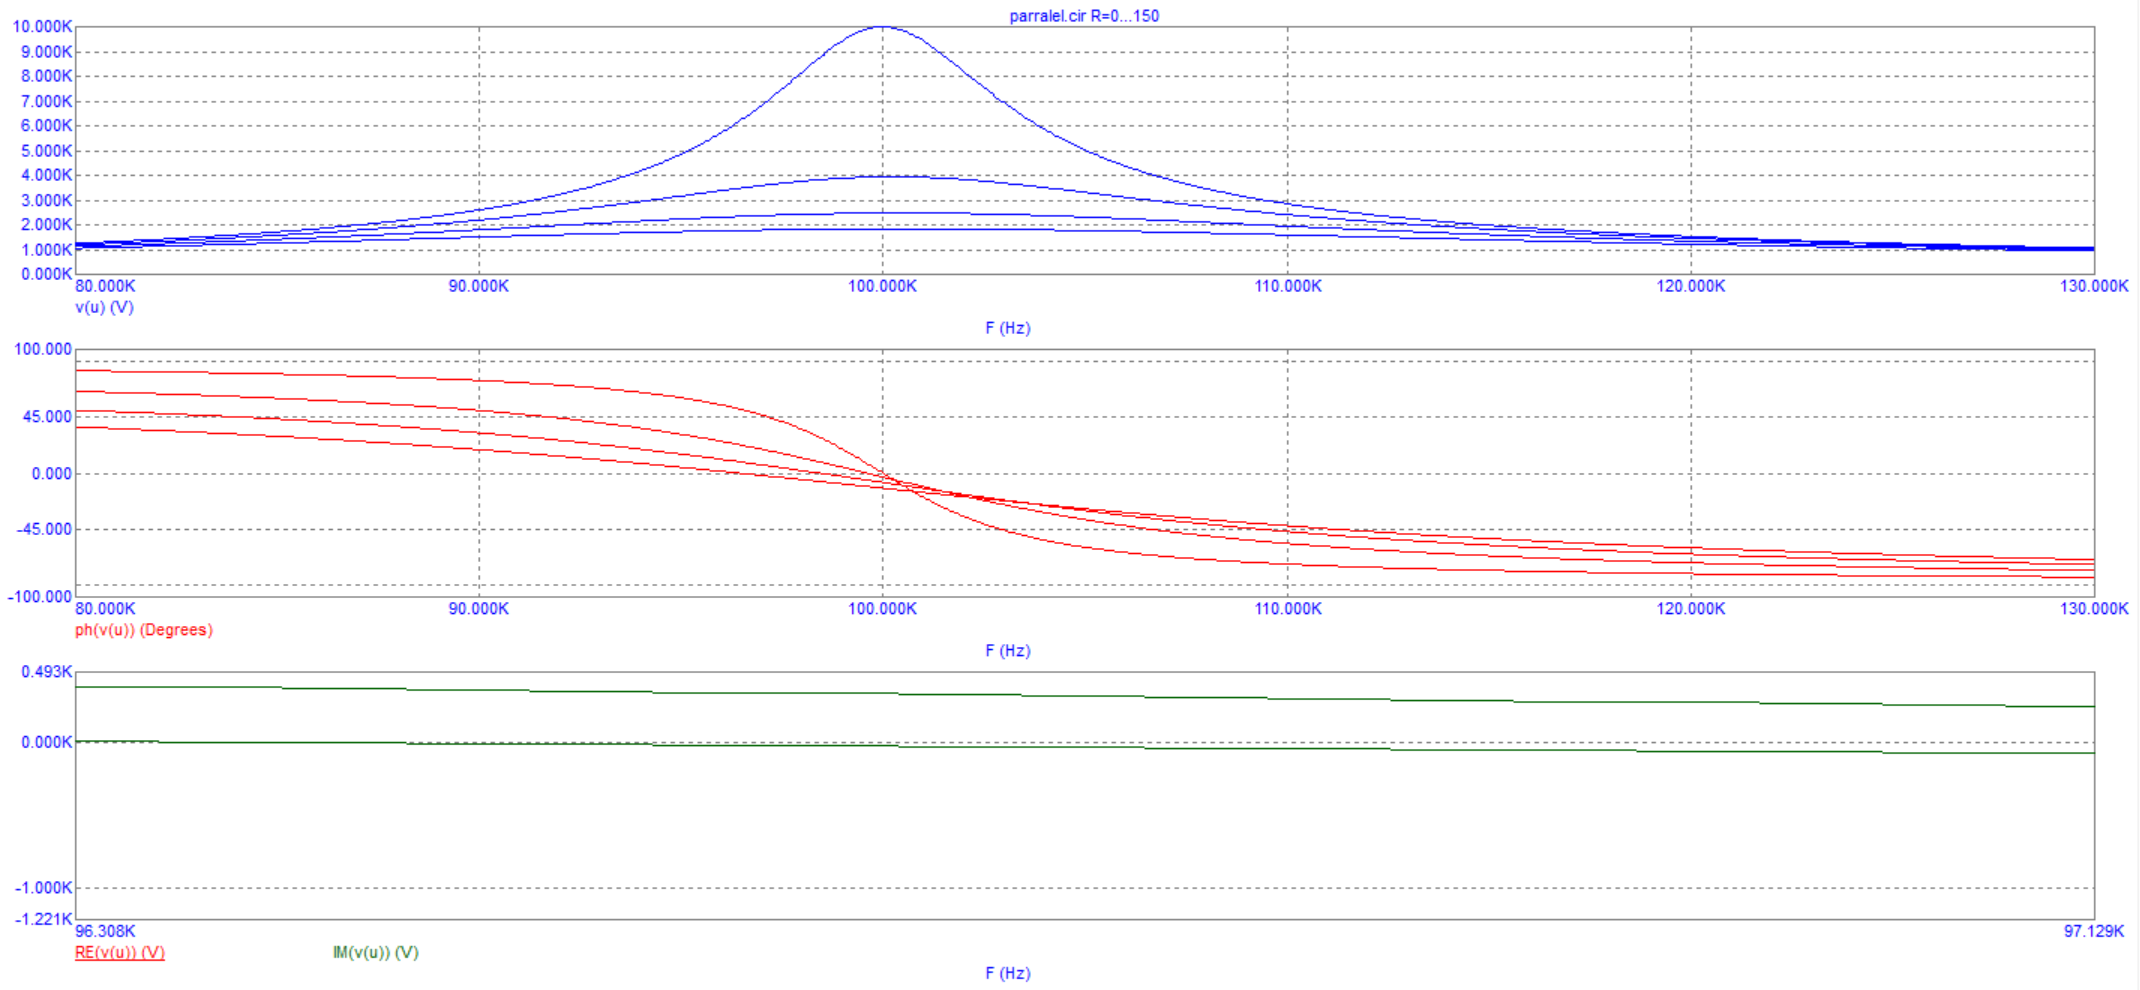
\includegraphics[scale=0.4]{parallel_AC2.png}
\label{fig:Image1}
\end{figure} 

\begin{center}
\begin{tabular}{|c|c|c|c|c|}
\hline 
$R, \: \textit{Ом}$ & 0 & 50 & 100 & 150 \\ 
\hline 
$f_{\textit{эксп}}, \: \textit{кГц}$ & 100 & 99,6 & 98,42 & 96,4 \\ 
\hline 
$\beta$ & 0 & 0,088 & 0,176 & 0,264 \\ 
\hline 
$f_{\textit{теор}}$ & 100 & 99,6 & 98,43 & 96,45 \\ 
\hline 
\end{tabular} 
\end{center}

\item Исследуем влияние последовательных потерь в области низких частот. Установим частотный диапазон от $1 \: \textit{кГц}$ до $130 \: \textit{кГц}$ и будем варьировать $R = [0,20 \Vert 2]$.

\begin{figure}[h!]
\centering
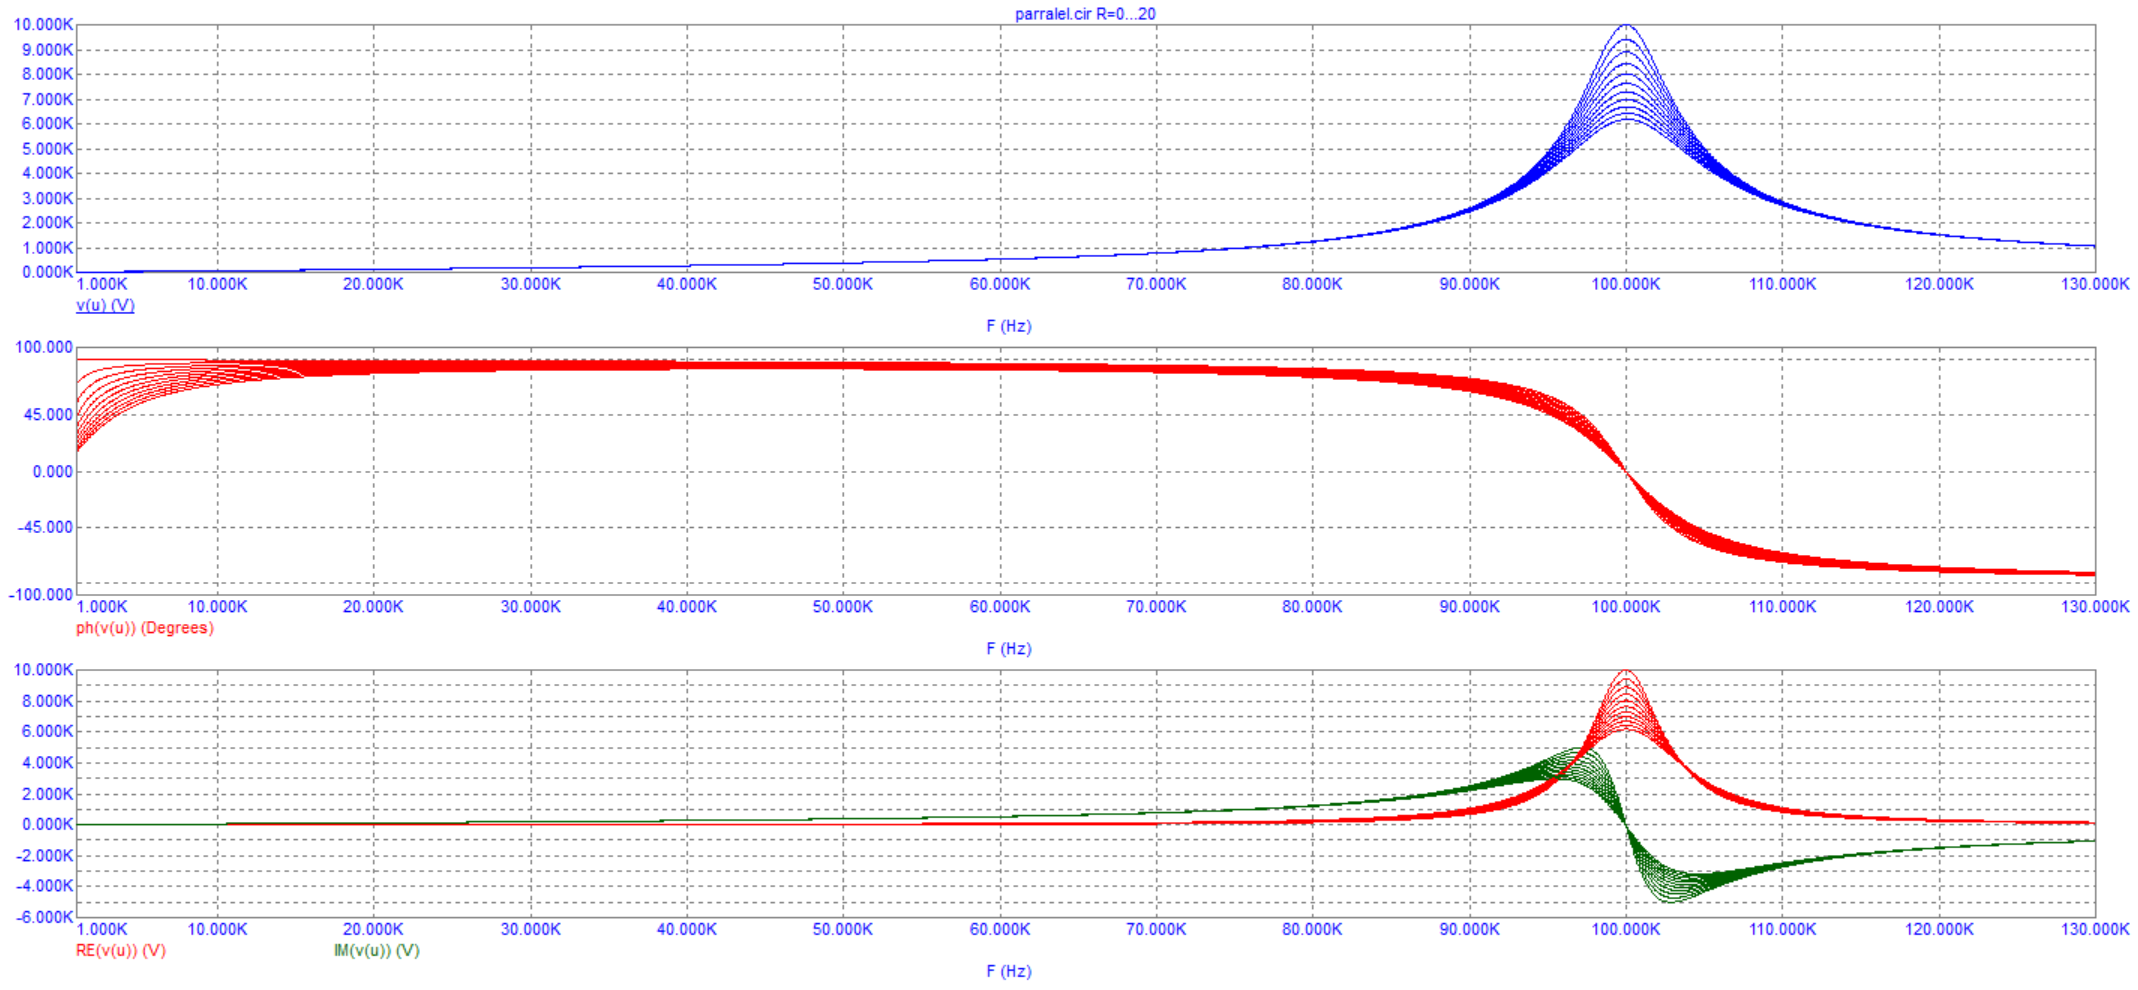
\includegraphics[scale=0.4]{parallel_AC3.png}
\label{fig:Image1}
\end{figure} 

Получаем, что при $R = 12 \: \textit{Ом}$ фазовый сдвиг на частоте $f = 2 \: \textit{кГц}$ составляет $\pi / 4$. 

\end{enumerate}

\section*{ЗАДАНИЕ 6}

\begin{enumerate}

\item Откроем модель \textbf{combined.cir} с $f_0 = 100 \: \textit{кГц}$, $\rho = 15,9 \: \textit{кГц}$, $q \simeq 10$, $\alpha = 1$.

\begin{figure}[h!]
\centering
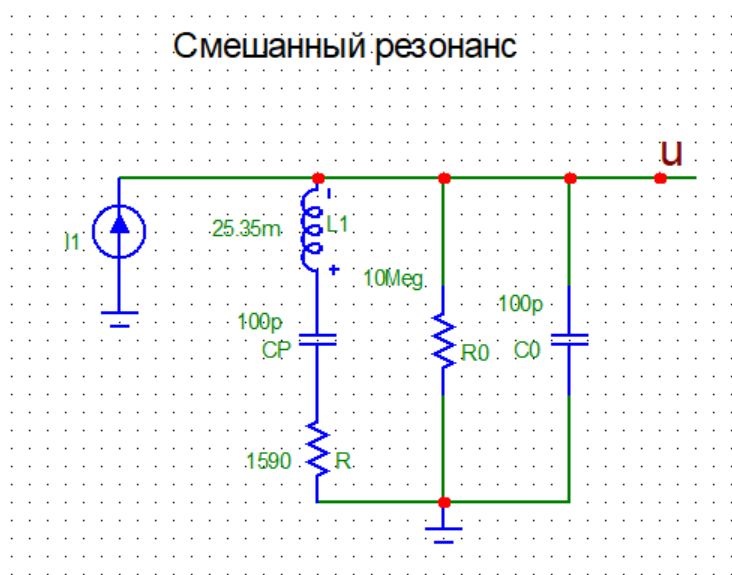
\includegraphics[scale=0.4]{combined_img.png}
\label{fig:Image1}
\end{figure}

Изучим графики частотной и фазовой характеристик, а также графики частотных зависимостей вещественной и мнимой частей мпеданса.

\begin{figure}[h!]
\centering
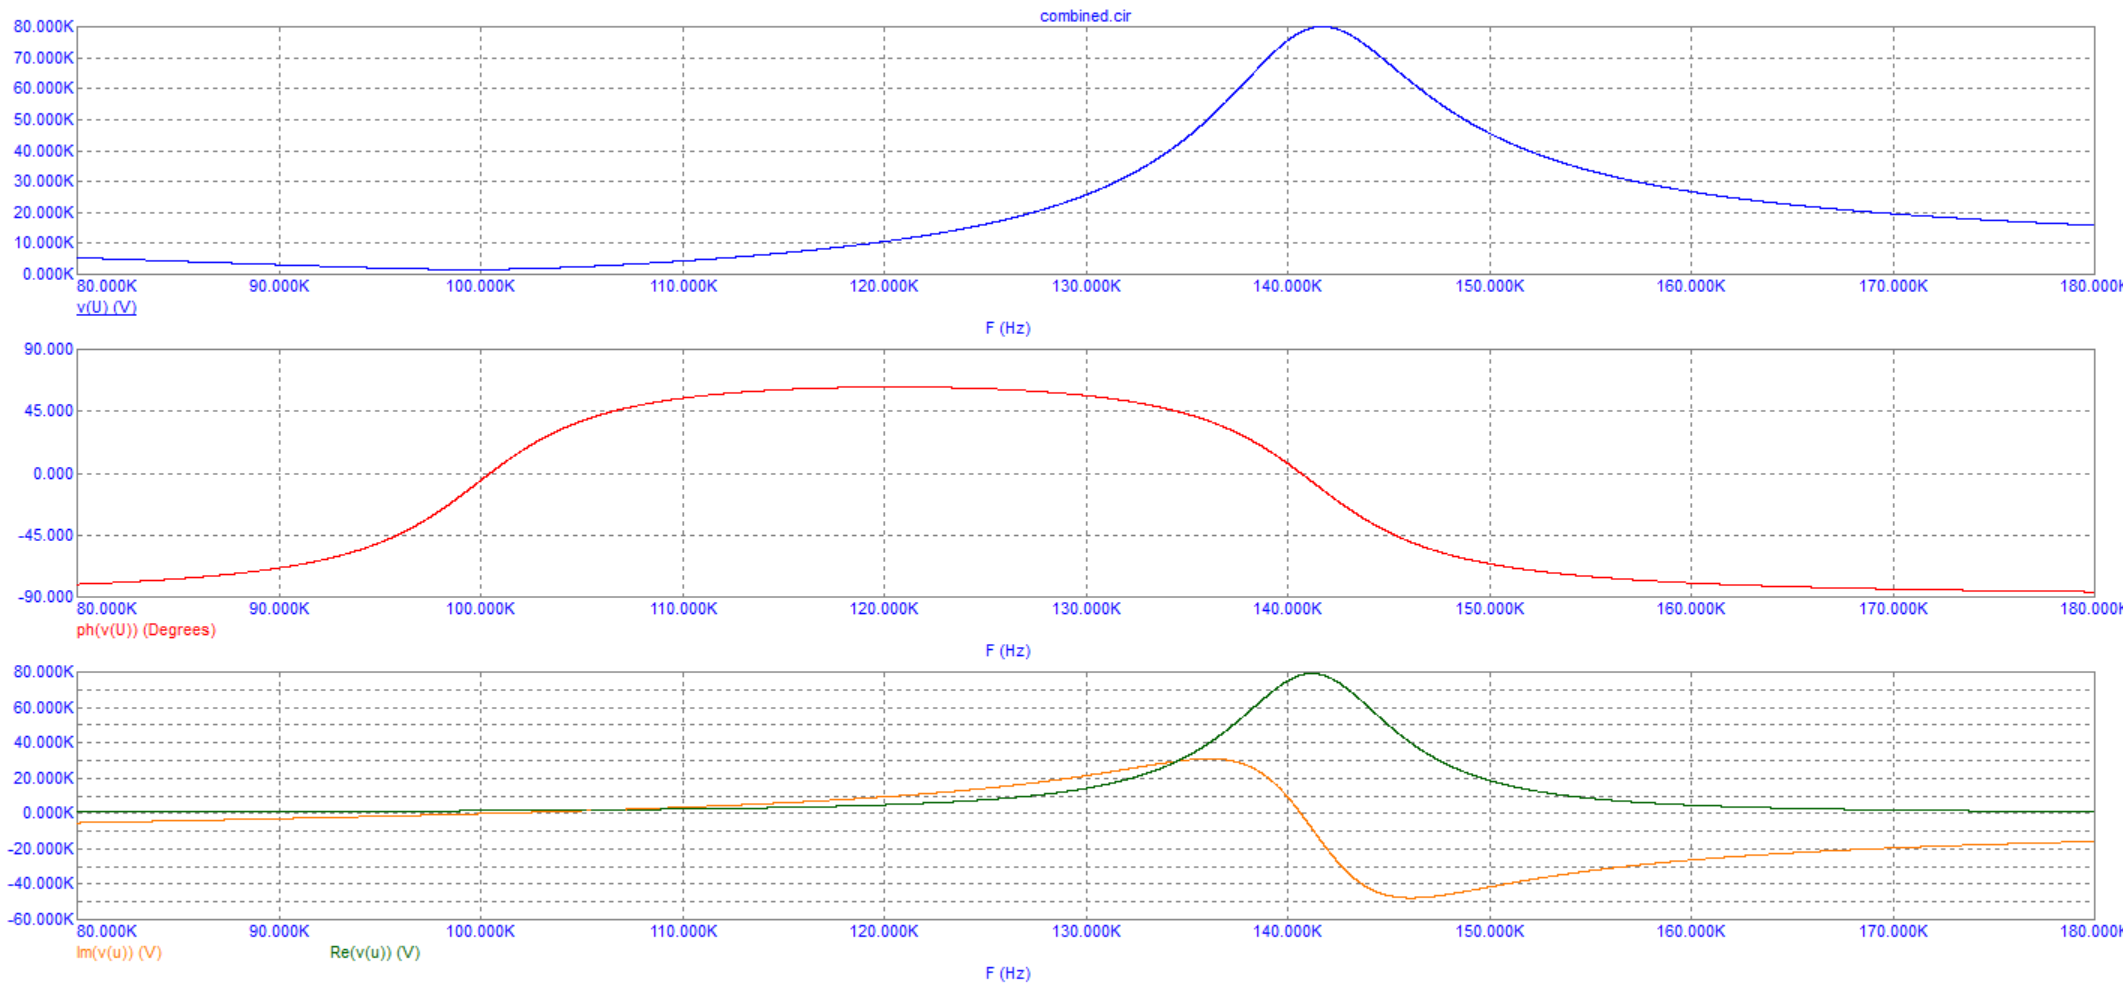
\includegraphics[scale=0.4]{combined_AC1.png}
\label{fig:Image1}
\end{figure}

\item Измерим частоты $f_p, f_0$ последовательного и параллельного резонансов по точкам пересечения нуля фазовой характеристикой:

\[f_p = 100,5 \: \textit{кГц} \quad f_0 = 140,6 \: \textit{кГц}\]

Измерим полосы $\triangle f_p, \triangle f_0$, в которых фазовая характеристика изменяется в диапазоне $\pm 45 \deg$ в окрестностях резонансов.

\[\triangle f_p = 10,6 \: \textit{кГц}\]

\[\triangle f_0 = 10,8 \: \textit{кГц}\]

Оценим добротности $Q_p, Q_0$ и проверим, что $f_0 = f_p \sqrt{2}$, $Q_0 = Q_p \sqrt{2}$:

\[Q_p = \frac{f_p}{\triangle f_p} = 9,5\]

\[Q_0 = \frac{f_0}{\triangle f_0} = 13\]

\[Q_0 = 13 \simeq 13,43 = Q_p \sqrt{2}\]

\[f_0 = 140,6 \simeq 142,1 = f_p \sqrt{2}\]

\item Измерим сопротивление контура на частотах последовательного и параллельного резонансов, сравним результаты с теоретическими значениями ($r, k^2\rho_p, Q_p$):

\[r_{\textit{эксп}} = 1,565 \: \textit{кОм} \simeq 1,59 \: \textit{кОм} = r_{\textit{теор}}\]

\[(k^2\rho_p, Q_p)_{\textit{эксп}} = 78,1 \: \textit{кОм} \simeq  79,1 \: \textit{кОм} = \Big(\frac{\alpha}{1 + \alpha}\Big)^2 \sqrt{\frac{L}{c}}(1 + \alpha)\frac{r}{\rho} = (k^2\rho_p, Q_p)_{\textit{теор}}\]

Снимем зависимость сопротивления на частоте параллельного резонанса от $R = [500, 2000 \Vert 500]$ и емкости $C_0 = [100p, 300p \Vert 100p]$. Сопоставим их с теорией. Осмыслим характер изменения графиков при варьировании $R$ и $C_0$.

\begin{figure}[h!]
\centering
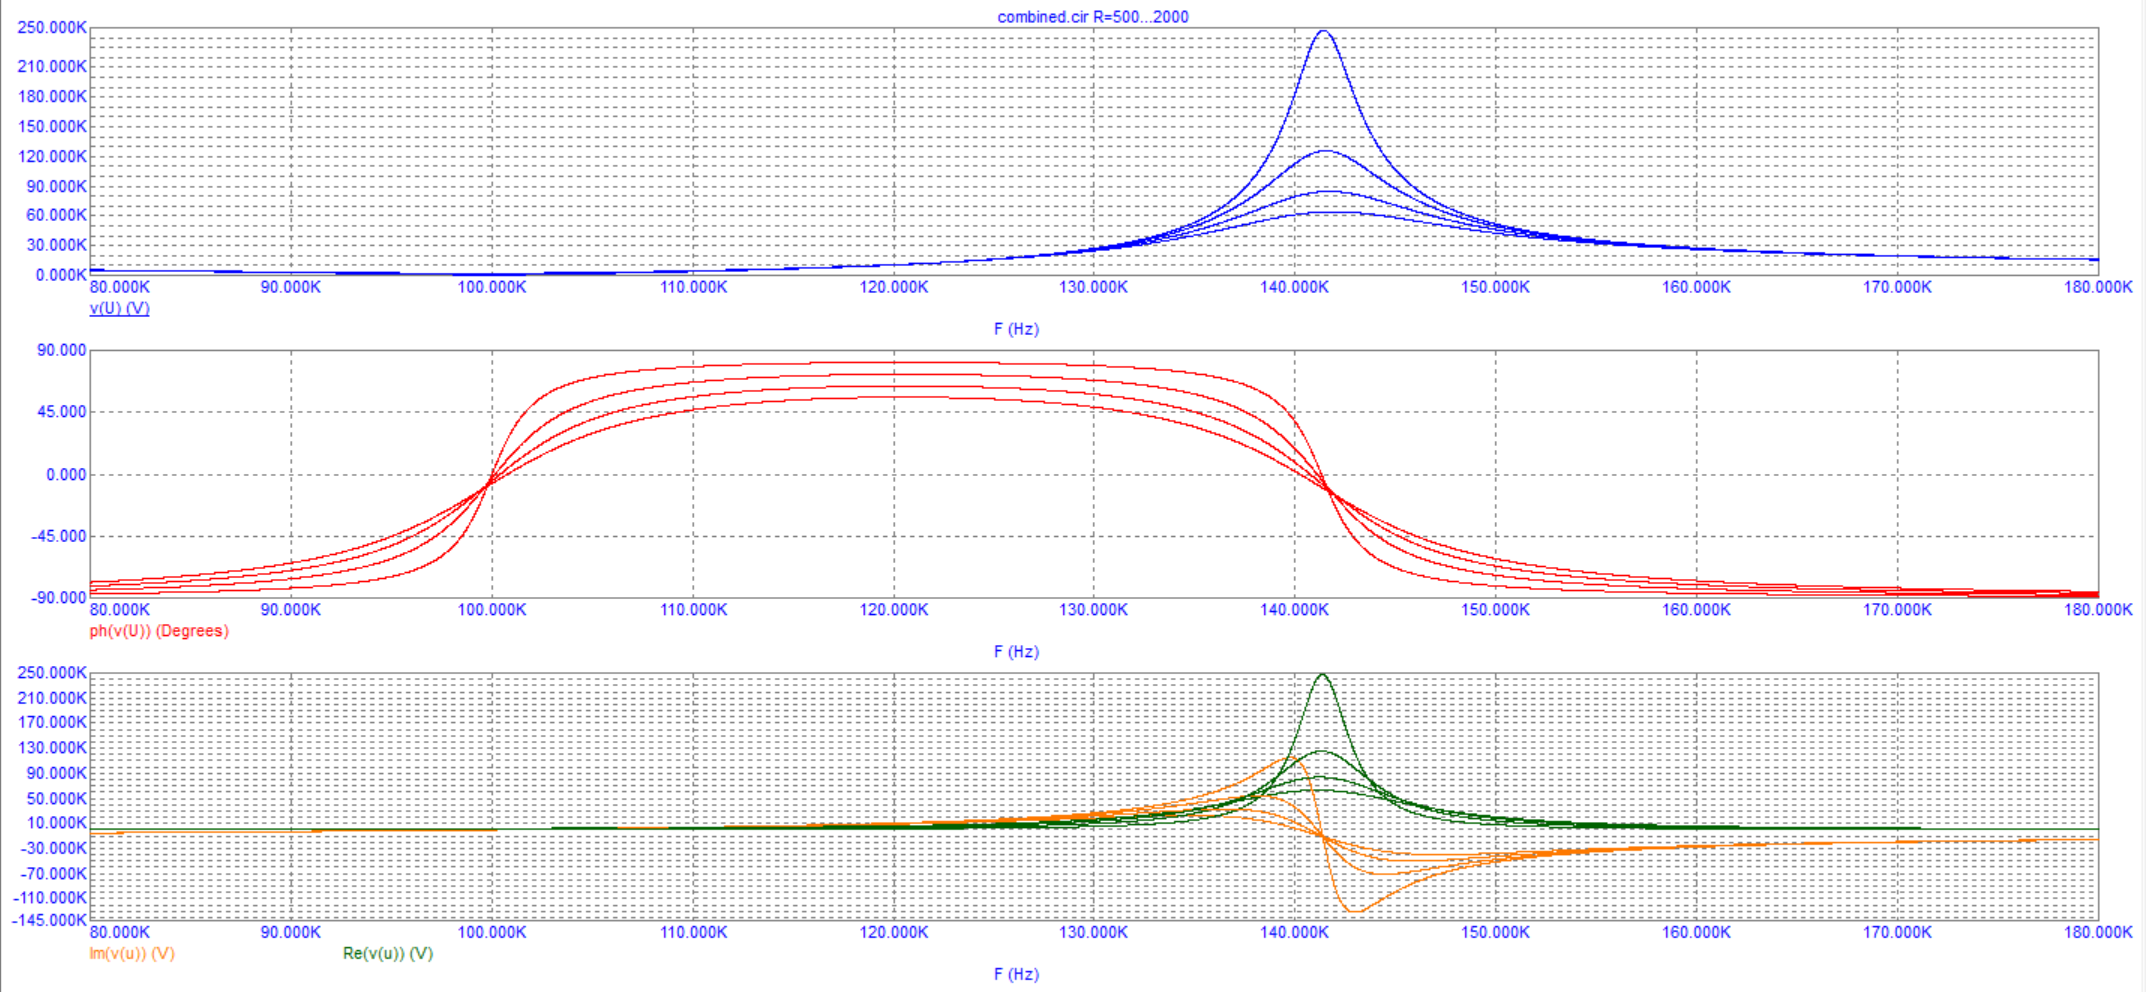
\includegraphics[scale=0.4]{combined_AC2.png}
\label{fig:Image1}
\end{figure}

\begin{center}
\begin{tabular}{|c|c|c|c|c|}
\hline 
$R, \: \textit{Ом}$ & 500 & 1000 & 1500 & 2000 \\ 
\hline 
$Z, \: \textit{кОм}$ & 247 & 124,4 & 83 & 61,9 \\ 
\hline 
\end{tabular} 
\end{center}

Получаем зависимость:

\[Z \sim \frac{1}{R}\]

\begin{figure}[h!]
\centering
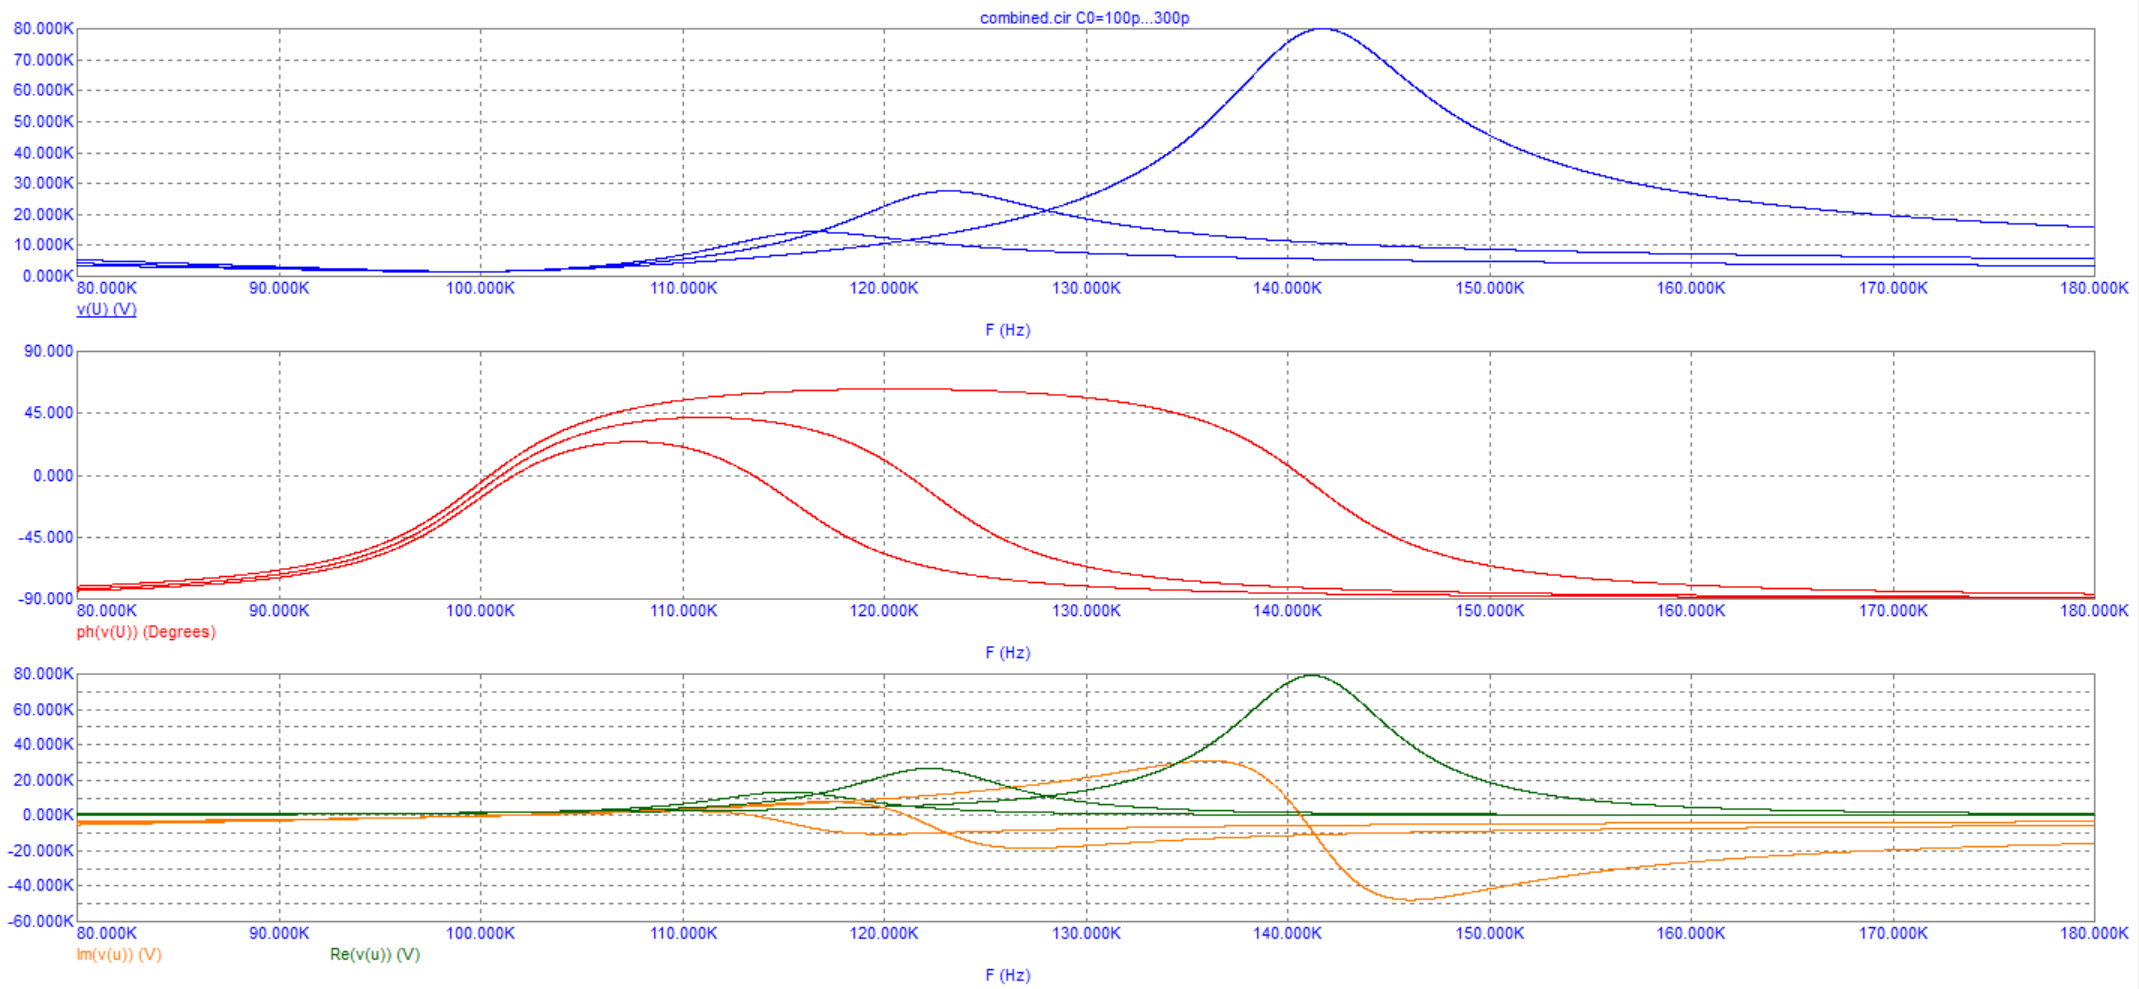
\includegraphics[scale=0.4]{combined_AC3.png}
\label{fig:Image1}
\end{figure}

\begin{center}
\begin{tabular}{|c|c|c|c|}
\hline 
$C_0, \: \textit{пФ}$ & 100 & 200 & 300 \\ 
\hline 
$Z, \: \textit{кОм}$ & 78,3 & 25,4 & 11,9 \\ 
\hline 
\end{tabular} 
\end{center}

Получаем зависимость:

\[Z \sim \frac{1}{C_0^2}\]

\item Обнулим последовательности потери $r$ и варьированием $R_0 = [10k, 100k \Vert 10k]$ подберем сопротивления параллельных потерь так, чтобы достичь того же резонансного сопротивления, что и при $r = 1590 \: \textit{Ом}$.

\begin{figure}[h!]
\centering
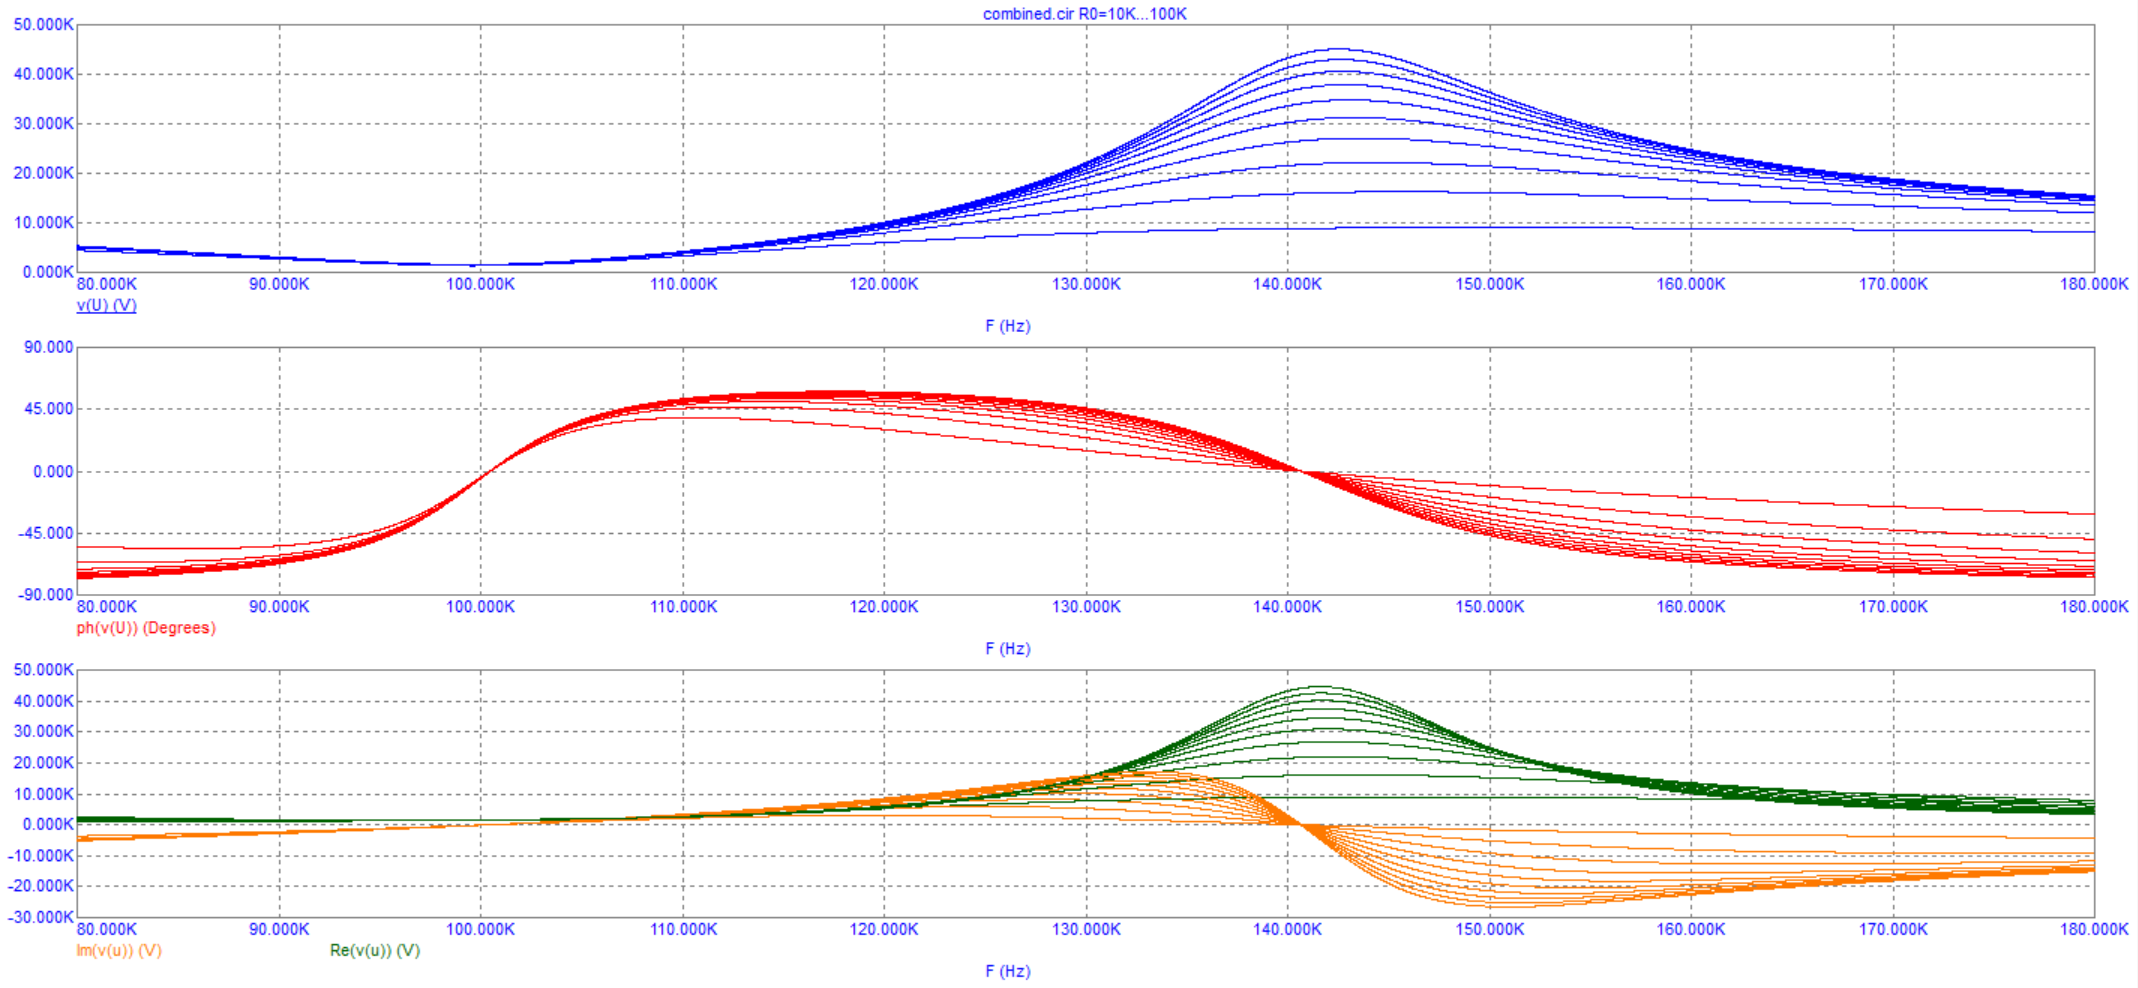
\includegraphics[scale=0.4]{combined_AC4.png}
\label{fig:Image1}
\end{figure}

Получим $R_0 = 80 \: \textit{кОм}$. Проверим закон пересчета:

\[R_0 r = k^2 \rho_p^2\]

\[80000 \cdot 1590 \simeq \Big(\frac{1}{2}\Big)^2 \cdot 2 \cdot 15900^2.\]

Соотношение выше выполняется.

\item Варьируя $R_0 = [80k, 10Meg \Vert 10Meg]$ при $r = 1590 \: \textit{Ом}$, изучим влияние $R_0$ на поведения частотной и фазовой характеристик на низких частотах - в диапазоне $1k, 180k$.

\begin{figure}[h!]
\centering
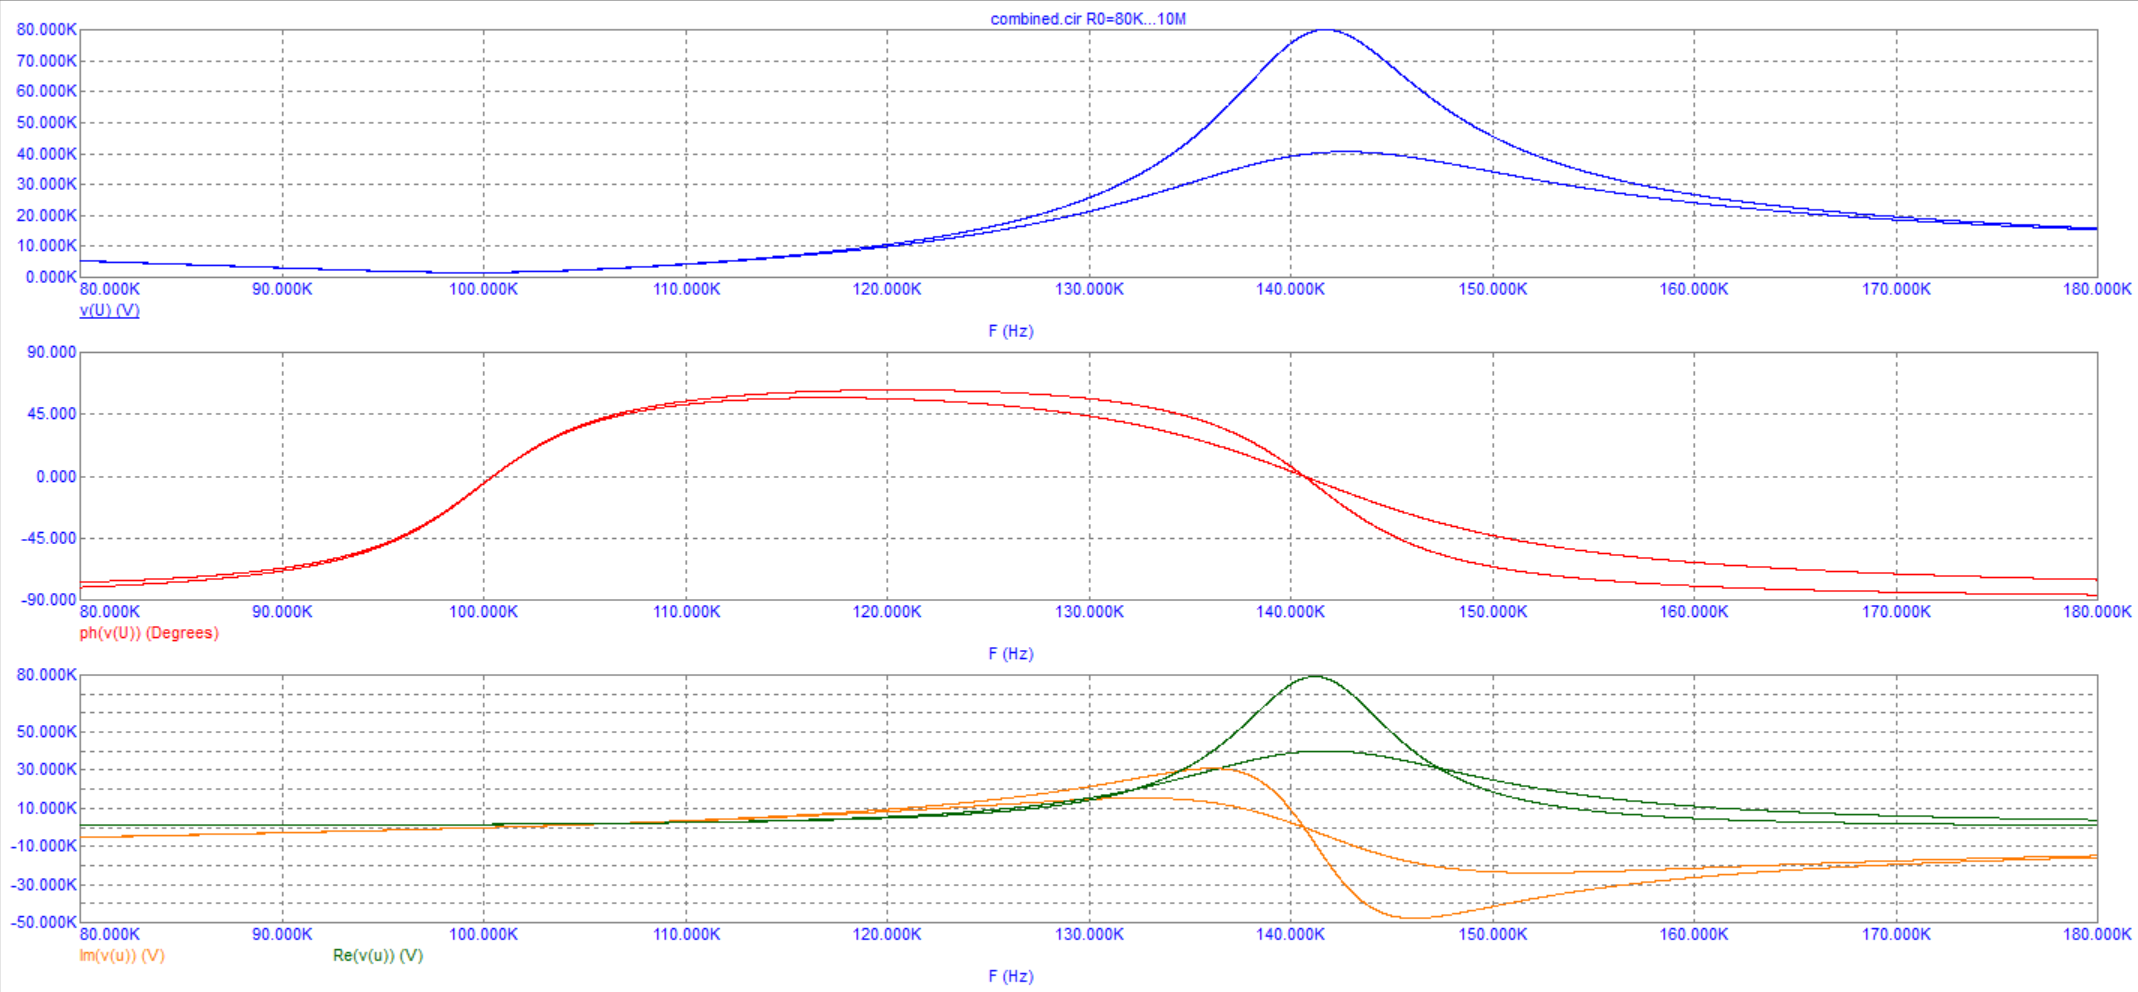
\includegraphics[scale=0.4]{combined_AC5.png}
\label{fig:Image1}
\end{figure}

При увеличении $R_0$ частотная характеристика увеличивается, а фазовая уменьшается.

\end{enumerate}

\end{document}